\documentclass[12pt, a4paper, oneside]{Thesis} % Paper size, default font size and one-sided paper
\usepackage{wrapfig}
\usepackage{lscape}
\usepackage{rotating}
\usepackage{graphicx}
\usepackage{caption}
\usepackage{amsmath}
\usepackage[boxed]{algorithm}
\usepackage[noend]{algpseudocode}



\usepackage{lineno,hyperref}
\modulolinenumbers[5]


\usepackage{amssymb}
\usepackage{graphicx}
\usepackage{array}
\usepackage{float}
\usepackage{placeins}
\usepackage{stackengine}
\usepackage{url}
\usepackage{numprint}
\usepackage{caption}

\usepackage{booktabs}  
\usepackage{siunitx}
%\usepackage[showframe=false]{geometry}
\usepackage{subfigure}

\nprounddigits{3}
\newcolumntype{P}[1]{>{\centering\arraybackslash}p{#1}}
\newcolumntype{M}[1]{>{\centering\arraybackslash}m{#1}}

\setstackEOL{\#}
\setstackgap{L}{12pt}


%\usepackage{subcaption} %incompatible with subfig
\graphicspath{{Pictures/}} % Specifies the directory where pictures are stored
\usepackage[numbers,square]{natbib} % Use the natbib reference package - read up on this to edit the reference style; if you want text (e.g. Smith et al., 2012) for the in-text references (instead of numbers), remove 'numbers' v

\hypersetup{urlcolor=black, colorlinks=false} % Colors hyperlinks in blue - change to black if annoyingv`	

\thesistitle{PySchedCL: A Framework for Automatically Exploiting Concurrency in Heterogeneous Data-Parallel Applications}
\supervisor{Professor Soumyajit Dey}
\degree{Dual Degree (B.Tech + M.Tech)}
\degreemajor{Computer Science and Engineering}
\authors{Siddharth Singh}
\rollno{15CS30032}
\university{Indian Institute of Technology Kharagpur}
\department{Department of Computer Science and Engineering}
\unisite{http://www.iitkgp.ac.in}
\depsite{http://cse.iitkgp.ac.in/}
\placeshrt{Kharagpur}
\placelng{Kharagpur - 721302, India}
\datesub{June 2, 2020}
\datesig{June 2, 2020}
\semsub{Spring Semester, 2019-20}
\keywords{High Performance Computing}
\coursecd{M.Tech Project - II Thesis }

\title{\ttitle} % Defines the thesis title - don't touch this
\begin{document}
%\makeatletter
%\renewcommand*{\NAT@nmfmt}[1]{\textsc{#1}}
%\makeatother

% prints author names as small caps


\frontmatter % Use roman page numbering style (i, ii, iii, iv...) for the pre-content pages

\setstretch{1.6} % Line spacing of 1.6 (double line spacing)

% Define the page headers using the FancyHdr package and set up for one-sided printing
\fancyhead{} % Clears all page headers and footers
\rhead{\thepage} % Sets the right side header to show the page number
\lhead{} % Clears the left side page header

%\pagestyle{fancy} % Finally, use the "fancy" page style to implement the FancyHdr headers

\newcommand{\HRule}{\rule{\linewidth}{0.5mm}} % New command to make the lines in the title page

% PDF meta-data
\hypersetup{pdftitle={\ttitle}}
\hypersetup{pdfsubject=\subjectname}
\hypersetup{pdfauthor=\authornames}
\hypersetup{pdfkeywords=\keywordnames}

%----------------------------------------------------------------------------------------
%	TITLE PAGE
%----------------------------------------------------------------------------------------
\maketitle
%\titlepg % Add a gap in the Contents, for aesthetics

\clearpage % Start a new page

%----------------------------------------------------------------------------------------
%	DECLARATION PAGE
%	Your institution may give you a different text to place here
%----------------------------------------------------------------------------------------


\Declaration% Add a gap in the Contents, for aesthetics


%----------------------------------------------------------------------------------------
%	CERTIFICATE PAGE
%----------------------------------------------------------------------------------------

\addtotoc{Certificate} % Add the "Abstract" page entry to the Contents

\certificate{\addtocontents{toc}{} % Add a gap in the Contents, for aesthetics

\clearpage % Start a new page

%----------------------------------------------------------------------------------------
%	ABSTRACT PAGE
%----------------------------------------------------------------------------------------

\addtotoc{Abstract} % Add the "Abstract" page entry to the Contents

\abstract{\addtocontents{toc}{} % Add a gap in the Contents, for aesthetics
% The past decade has seen diminishing returns from Moore's Law because of increasing fabrication costs,
% technological barriers and power density limits. As a result Heterogeneous Computing architectures (like multi-core CPUs with a GPU) have been adopted almost universally to optimise performance. 
% These architectures have been complemented well by parallel programming languages like CUDA and OpenCL which have been used to build several high performance solutions in a diverse set of fields.
% The focus of this thesis is the latter i.e. OpenCL, due to it being the most pervasive, cross-vendor, open standard for heterogenous parallel programming. 
% Inspite of the ubiquitous nature of heterogenous computing, programmers require a considerable amount of expertise to efficiently design data parallel algorithms. Further, due to the low level nature of OpenCL, there is a lot of programming 
% overhead to ensure correctness during execution and data transfer via synchornisation. The primary aim of 
% our framework - PyschedCL is to address the above issues in designing OpenCL applications and help a novice
% end user bridge the gap between homogenous and heterogenous computing systems. It completely eliminates the programming overhead by automating 
% the synchornisation routines to ensure correctness. The scheduling backend also comprises of a Machine Learning based 
% scheduling policy which can intelligently map the underlying elements of an application to the target heterogenous platform. The modular nature of the framework allows the user to 
% replace the scheduling policy of the backend with a custom scheduling algorithm too. This can help researchers design and validate several scheduling algorithms. The framework tries to exploit 
In the past decade, high performance compute capabilities exhibited by heterogeneous GPGPU platforms have led to the popularity of  data parallel programming languages such as CUDA and OpenCL. Such languages, however,  involve a steep learning curve as well as developing an extensive understanding of the underlying architecture of the compute devices in heterogeneous platforms. This has led to the emergence of several High Performance Computing frameworks which provide high-level abstractions for easing the development of data-parallel applications on heterogeneous platforms. However, the scheduling decisions undertaken by such frameworks do not sufficiently exploit the concurrency inherent in a data parallel application to its full potential. We propose a framework called {\em PySchedCL}, whose design philosophy is along similar lines as that of other HPC frameworks, with a specific focus on exploring fine-grained concurrency aware scheduling decisions that completely harness the power of heterogeneous CPU/GPU architectures. We showcase the efficacy of such scheduling decisions over popular dynamic scheduling schemes by conducting extensive experimental evaluations for a Machine Learning based inferencing application. We also experiment with automated coarse-grained scheduling algorithm that rely on Machine learning to schedule heterogenous applications. 


}

\clearpage % Start a new page



%----------------------------------------------------------------------------------------
%	ACKNOWLEDGEMENTS
%----------------------------------------------------------------------------------------

\setstretch{1.3} % Reset the line-spacing to 1.3 for body text (if it has changed)

\acknowledgements{\addtocontents{toc}{}%\vspace{1em}} % Add a gap in the Contents, for aesthetics

I am deeply grateful to my supervisor \textbf{Prof. Soumyajit Dey} who gave me the opportunity to work on this project. I am thankful for his aspiring guidance, invaluably constructive friendly advice during the course of the project. I am sincerely grateful to him for sharing his truthful and illuminating views on a number of issues related to the project. I owe a lot to my teachers in the Department of Computer Science and Engineering, Indian Institute of Technology, Kharagpur, who have instilled in me the scientific spirit of inquiry, experimentation, observation and inference, without which I would not have been able to produce this work. Also, I am very thankful to \textbf{Mr. Anirban Ghose} involved in this project who constantly motivated me to overcome all the challenges and helped me whenever I faced any issues.


}
\clearpage % Start a new page

%----------------------------------------------------------------------------------------
%	LIST OF CONTENTS/FIGURES/TABLES PAGES
%----------------------------------------------------------------------------------------

\pagestyle{fancy} % The page style headers have been "empty" all this time, now use the "fancy" headers as defined before to bring them back

\lhead{\emph{Contents}} % Set the left side page header to "Contents"
\tableofcontents % Write out the Table of Contents

\lhead{\emph{List of Figures}} % Set the left side page header to "List of Figures"
\listoffigures % Write out the List of Figures

\lhead{\emph{List of Tables}} % Set the left side page header to "List of Tables"
\listoftables % Write out the List of Tables

%----------------------------------------------------------------------------------------
%	ABBREVIATIONS
%----------------------------------------------------------------------------------------

% \clearpage % Start a new page

% \setstretch{1.5} % Set the line spacing to 1.5, this makes the following tables easier to read

% \lhead{\emph{Abbreviations}} % Set the left side page header to "Abbreviations"
% \listofsymbols{ll} % Include a list of Abbreviations (a table of two columns)
% {
% \textbf{FEA} & \textbf{F}inite \textbf{E}lement \textbf{A}nalysis \\
% \textbf{FEM} & \textbf{F}inite \textbf{E}lement \textbf{M}ethod \\
% \textbf{LVDT} & \textbf{L}inear \textbf{V}ariable \textbf{D}ifferential \textbf{T}ransformer \\
% \textbf{RC} & \textbf{R}einforced \textbf{C}oncrete
% %\textbf{Acronym} & \textbf{W}hat (it) \textbf{S}tands \textbf{F}or \\
% }

%----------------------------------------------------------------------------------------
%	PHYSICAL CONSTANTS/OTHER DEFINITIONS
%----------------------------------------------------------------------------------------
%
%\clearpage % Start a new page
%
%\lhead{\emph{Physical Constants}} % Set the left side page header to "Physical Constants"
%
%\listofconstants{lrcl} % Include a list of Physical Constants (a four column table)
%{
%Speed of Light & $c$ & $=$ & $2.997\ 924\ 58\times10^{8}\ \mbox{ms}^{-\mbox{s}}$ (exact)\\
%% Constant Name & Symbol & = & Constant Value (with units) \\
%}

%----------------------------------------------------------------------------------------
%	SYMBOLS
%----------------------------------------------------------------------------------------

% \clearpage % Start a new page

% \lhead{\emph{Symbols}} % Set the left side page header to "Symbols"

% \listofnomenclature{lll} % Include a list of Symbols (a two column table)
% {
% $D^{el}$ & elasticity tensor \\
% $\sigma$ & stress tensor \\
% $ \varepsilon $ & strain tensor \\
% % Symbol & Name & Unit \\

% }

%----------------------------------------------------------------------------------------
%	DEDICATION
%----------------------------------------------------------------------------------------
%
%\setstretch{1.3} % Return the line spacing back to 1.3
%
%\pagestyle{empty} % Page style needs to be empty for this page
%
%\dedicatory{For/Dedicated to/To my\ldots} % Dedication text
%
%\addtocontents{toc}{\vspace{2em}} % Add a gap in the Contents, for aesthetics

%----------------------------------------------------------------------------------------
%	THESIS CONTENT - CHAPTERS
%----------------------------------------------------------------------------------------

\mainmatter % Begin numeric (1,2,3...) page numbering

\pagestyle{fancy} % Return the page headers back to the "fancy" style

% Include the chapters of the thesis as separate files from the Chapters folder
% Uncomment the lines as you write the chapters

% Chapter Template

\chapter{Introduction} % Main chapter title

\label{Chapter 1} % Change X to a consecutive number; for referencing this chapter elsewhere, use \ref{ChapterX}

\lhead{Chapter 1. \emph{Introduction}} % Change X to a consecutive number; this is for the header on each page - perhaps a shortened title

%----------------------------------------------------------------------------------------
%	SECTION 1
%---------------------------------------------------------------------------------------
\section{Introduction}

% Chapter Template

\chapter{OpenCL Background and Related Work} % Main chapter title

\label{Chapter2} % Change X to a consecutive number; for referencing this chapter elsewhere, use \ref{ChapterX}

\lhead{Chapter 2. \emph{OpenCL Background and Related Work}} % Change X to a consecutive number; this is for the header on each page - perhaps a shortened title

%----------------------------------------------------------------------------------------
%	SECTION 1
%----------------------------------------------------------------------------------------

\section{OpenCL Background}

Any OpenCL application typically comprises two distinct program entities - i) the {\em host} which is a single threaded sequential program executing on one CPU core that orchestrates the entire process of managing data and issuing directives for parallel execution, and ii) kernel(s) which execute on devices with support for vector processing (CPU,GPU,FPGA,DSP).  For every computational kernel, the single-threaded host program leverages command queues supported by the OpenCL API to issue commands for  performing the following operations - i) copying the data from host to input buffers resident on device memory (Host to Device or H2D transfer), ii) launching multiple instances of the same kernel to process the data copied to the device and iii) copying back the data stored in output buffers in the device after the kernel has finished processing back to the host memory (Device to Host or D2H transfer). 
	\par As an illustrative example, we consider a simple OpenCL application which performs a vector addition followed by an element-wise trigonometric sine operation. The vector addition kernel $vadd$ executes on device $GPU_0$. It takes as input two input buffers ($b0$ and $b1$) performs element-wise addition and produces an output buffer ($b2$). The kernel $vsin$ executes on device $GPU_1$ and takes one buffer ($b3$) and performs an inplace element-wise sine operation. In Fig. \ref{fig:OpenCLArch}, the OpenCL host program sets up command queues for each GPU device. For $GPU_0$, the host first issues two {\em write} commands ({\tt clEnqueueWrite()}) for buffers $b0$ and $b1$ followed by a {\em barrier} directive ({\tt clEnqueueBarrier()}). The {\em barrier} command in general ensures that all commands enqueued previously finish before proceeding to execute commands enqueued after the barrier. In this case, it is ensured that the write commands are finished before processing the next command in the queue. The host next issues one execute command ({\tt clEnqueueNDRangeKernel()})followed by a barrier directive and finally one read command ({\tt clEnqueueReadBuffer()}) followed again by a barrier directive. We note all the functions with the {\tt clEnqueue} prefix asynchronously issues these commands to the OpenCL runtime system i.e. the host does not have to explicitly wait for a particular command to finish. It simply enqueues the commands and is free to execute  something else while those commands are executed on the target device. 
	\begin{figure}[ht]  
		\centering
		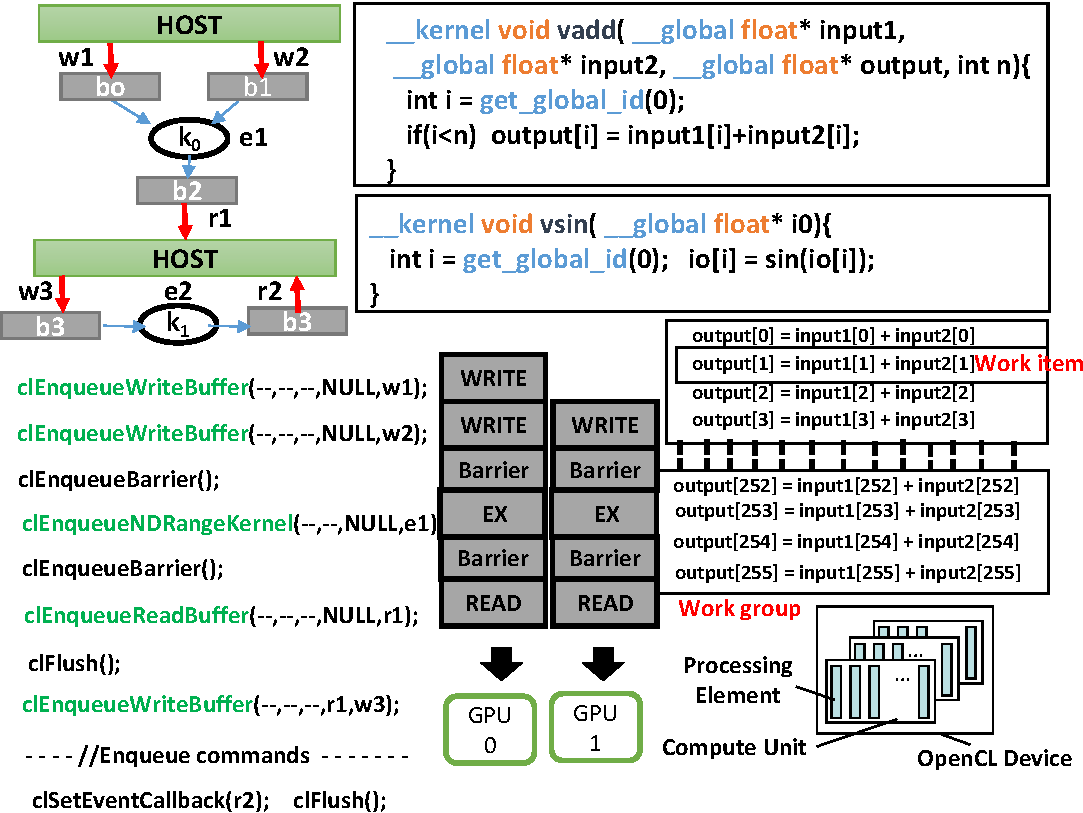
\includegraphics[scale=0.47]{Pictures/OpenCLBackground.pdf}
		\caption{OpenCL Execution \label{fig:OpenCLArch}}
	\end{figure}
	\par The command {\tt clEnqueueNDRangeKernel()} spawns a collection of threads referred as \textit{work items} where each work item executes on a \textit{processing element} on the heterogeneous platform. Each work item is referred by a unique identifier $i$ obtained using the {\tt get\_global\_id()} OpenCL function and is responsible for the addition of  data points in the two input buffers $b0$ and $b1$ ({\tt input1[i]} and {\tt input2[i]} in function call) and storing the result in the corresponding location of the output buffer ({\tt output[i]} in function call). Work items are further grouped into \textit{work groups} and each work group is scheduled for execution on a \textit{compute unit} in an OpenCL compliant device. A \textit{compute unit} may be a Symmetric Multiprocessor(SM) for a GPU device, a single core of a multicore CPU etc. 
	\par Similarly, it may be observed from Fig. \ref{fig:OpenCLArch}, the host issues a write command (for buffer $b3$), the execute command for $vsin$ kernel and one read command (for buffer $b3$ to the command queue pertaining to device $GPU_1$. We note that the write command for $vsin$ can start execution once the read command for the $vadd$ has finished. The OpenCL runtime system  has provisional APIs for specifying dependencies between commands. This is done using {\em events} which are objects that communicate the status of commands issued from the command queue. These events can be used for i) monitoring the execution of read/write operations and kernel execution, ii) enforcing dependencies across multiple commands and iii) notifying the host program about the completion of a command on the device. 
	\par In Fig. \ref{fig:OpenCLArch}, each \textit{write}, \textit{ndrange} and \textit{read} command $c$ enqueued is associated with an event $ev$. This is specified in the last argument of each command $c$ with {\tt clEnqueue} prefix. The second last argument of the function represents events on which the event $ev$ associated with command $c$ is dependent for execution. For our representative example, it may be observed that the event $w3$ is dependent on $r1$. This is specified in the {\tt clEnqueueWriteBuffer} command for buffer $w3$. This is followed by the other enqueue OpenCL function calls such as barriers,   launching the kernel and reading the final output buffer for $vsin$.   
	\par Finally, for the event associated with the last read command in the application (associated with event $r2$ in Fig. \ref{fig:OpenCLArch}), a \textit{callback function} is registered which is responsible for notifying the host when the computation has finished processing on a device. We note the {\tt clEnqueue} OpenCL functions merely enqueue operations to each command queue for the devices. After enqueuing all commands to a command queue, the function {\tt clFlush()} is invoked which informs the OpenCL runtime system to start dispatching the commands pushed to the command queue for execution.  
	\par OpenCL events are thus particularly useful for enforcing read/write and execute dependencies between multiple kernels in application task graphs which are typically represented by a directed acyclic graph (DAG) of OpenCL kernels.  %The state of the art frameworks (StarPU, MultiCL and SOCL) automate the process of setting up command queues and enqueuing commands for computational kernels allowing users to bypass the overhead of implementing boilerplate host code. However, the scheduling heuristics supported by these frameworks are optimized for GPGPU clusters comprising multiple compute nodes with heterogeneous CPU and GPU devices. The mapping decisions offered by these scheduling heuristics typically are coarse-grained in the sense that a single kernel can be mapped to a single device at a time. The supported heuristics do not leverage heuristics for concurrently executing multiple kernels on the same device. This can be achieved by setting up multiple OpenCL command queues on the same device and enqueuing respective write, execute and read commands. 
	We next discuss a slightly more complex DAG example and discuss how  coarse-grained and  fine-grained scheduling decisions result in different command queue configurations in the following subsection. 


\section{Related Work}
\par Given the rich API support by both heterogeneous programming models CUDA and OpenCL, several frameworks have emerged over the last few years with the objective of providing user friendly solutions for development of data parallel applications. Frameworks such as OpenACC \cite{openacc} supports a directive based programming model where relevant annotations in sequential C programs generate data parallel CUDA code for execution on the GPU. Similarly, the framework  HiCUDA \cite{hicuda} is another high level directive based programming language for generating CUDA binaries from sequential C source code. Frameworks such as GMAC \cite{gelado} offer a data centric programming model relieving the end designer from making explicit memory requests while implementing applications. We note that the frameworks discussed are built using the CUDA API and are restricted for use on heterogeneous systems with NVIDIA GPU architectures only. In constrast several OpenCL based frameworks have also been envisioned in the past decade for general purpose heterogeneous programming. 
	\par The most notable framework offering high-level abstractions for developing OpenCL applications is SkelCL \cite{skelCL} which offers algorithmic skeletons for developing data-parallel programs for execution across multiple GPUs. In this context, skeletons refer to higher order functions such as map, reduce, scan etc. which can be leveraged for implementing data parallel algorithms. Note, the primary approach of this work is complementary in the sense that they focus on rapid kernel development , while our work focuses on scheduling optimizations on target heterogeneous architectures. The VirtCL framework \cite{virtcl} provides an abstraction layer between the programmer and the OpenCL runtime system acting as a hypervisor for scheduling multiple OpenCL applications. The abstraction framework leverages a profile driven history based scheduling scheme for dispatching OpenCL kernels on multiple devices.   However a major limitation for VirtCL is that it cannot operate with devices belonging to different platforms. Our framework in contrast is suited to work with different OpenCL platforms and opts for a static based scheduling approach for mapping OpenCL kernels. There also exists frameworks such as SnUCL \cite{snucl}, VOCL \cite{vocl}, MultiCL \cite{multicl} etc. that extend upon the OpenCL runtime API that allow OpenCL applications to leverage devices belonging to heterogeneous clusters.  This work also presents a unified OpenCL implementation by incorporating a task queuing extension layer. However, such APIs still require explicit kernel and host program development and lack support for intelligent scheduling techniques mentioned earlier. 
	\par There also exist unified scheduling frameworks for heterogeneous platforms such as StarPU \cite{augonnet2011starpu} which provides users an interface for designing and experimenting scheduling policies for both CUDA and OpenCL applications. The StarPU runtime system allows users to design scheduling priority functions for experimentation. An extension on StarPU \cite{hugo2014composing} supports scheduling multiple tasks in parallel on a heterogeneous system.  The work reported in \cite{henry2014toward} presents an unified OpenCL implementation called SOCL which directly extends upon StarPU for handling and managing execution of OpenCL workloads across multiple devices using different scheduling policies. The SOCL API typically supports scheduling algorithms that require profiling information for each task on each device in the system beforehand. The most recent work in this domain is reported in \cite{pekka}, which proposes a set of APIs on top of OpenCL using which dependencies can be specified for application DAGs.
	\par Despite the vast number of frameworks available, our proposed framework relies on specification files using which programmers can bypass the overhead of implementing complex host programs and design data parallel applications with ease. We also present a novel software architecture that is capable of automatically extracting both application level and platform level concurrency. Currently the scheduling schemes lack support for performance models necessary for obtaining near-optimal schedules. Future work entails investigating machine learning assisted techniques \cite{grewe2011static,grewe2013opencl,kofler2013automatic,smart,schedcl} for the same. We believe the robust API support in our framework  would allow researchers to investigate these avenues and accordingly design and validate novel scheduling algorithms for heterogeneous platforms. 
% Chapter Template

\chapter{Problem Formulation} % Main chapter title

\label{Chapter3} % Change X to a consecutive number; for referencing this chapter elsewhere, use \ref{ChapterX}

\lhead{Chapter 3 \emph{Problem Formulation}} % Change X to a consecutive number; this is for the header on each page - perhaps a shortened title

\section{Motivation} \label{sec:motivation}
We consider a transformer application \cite{DBLP:journals/corr/VaswaniSPUJGKP17} which is a popular Deep Learning Neural Network pipeline for Natural Language Processing (NLP) tasks. The application exhibits ample scopes for exploiting concurrency with the possibility of executing multiple instances of standard General Matrix Multiply (GEMM) kernels in parallel. A sample DAG for one layer of the transformer network is presented in Fig. \ref{fig:motivation0}. We shall discuss necessary background and details about the workload later in the Experimental Results section.  
	\begin{figure}[ht]  
		\centering
		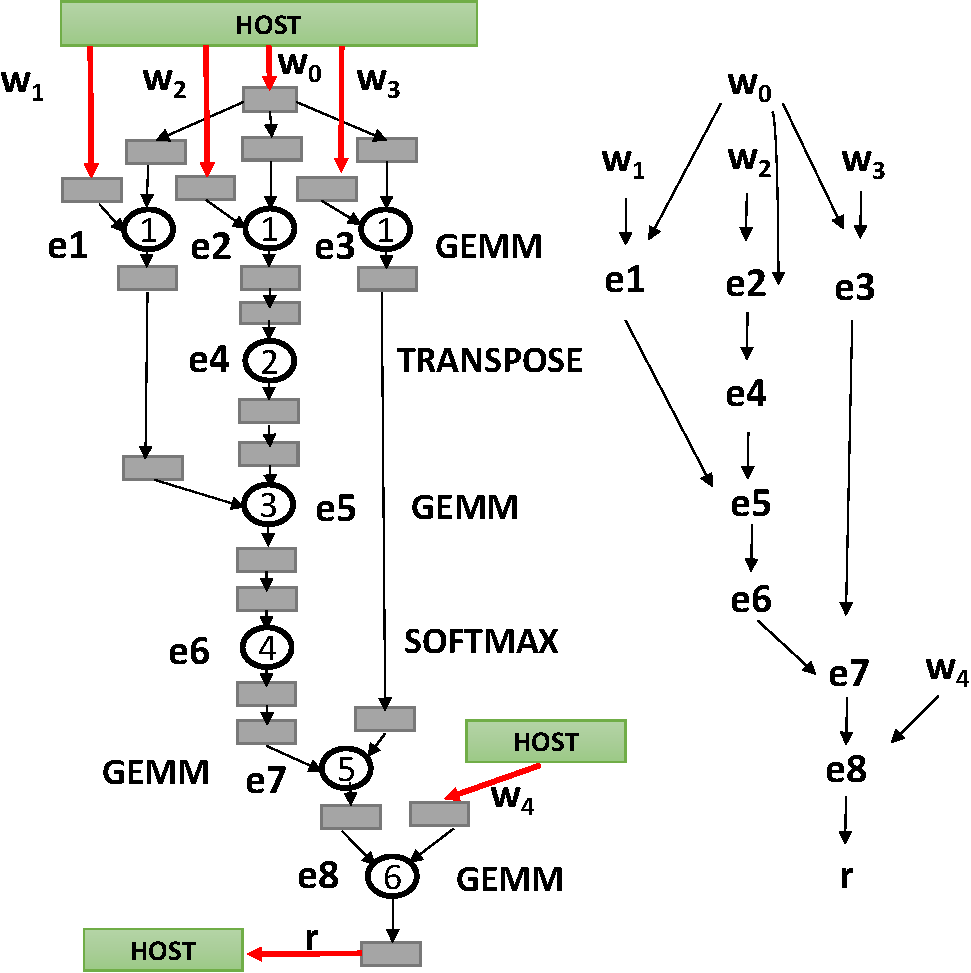
\includegraphics[scale=0.50]{Pictures/Transformer_modified.pdf}
		\caption{Event Dependencies for  DAG\label{fig:motivation0}}
	\end{figure}
	\par For the purpose of our motivation, we present a level wise view of the DAG under consideration  in the left hand side of Fig. \ref{fig:motivation0}, which contains a total of 8 kernels. As per our earlier convention, the rectangular nodes represent input output buffers and the circular nodes represent kernels Each kernel is labeled with the corresponding level number starting from 1. Initially there is a copy operation which copies the same buffer to each of the kernels at level 1.  Each of the kernels in levels 1,4,5,6 represent General Matrix Multiply (GEMM) kernels where each kernel takes as input two buffers and produces one output buffer. The kernels in level 2 and level 3 represent transpose and softmax operations respectively, each processing one input buffer to produce one output buffer. The edges between rectangular nodes i.e. buffers represent data dependencies for the DAG. For enforcing precedence constraints between any pair of  kernels $(k_i,k_j)$, a 
	programmer shall set event dependencies between read commands for output buffers of $k_i$ and write commands for input buffers of $k_j$, as was observed in Fig. \ref{fig:OpenCLArch}.  
	For our transformer DAG depicted in Fig. \ref{fig:motivation0}, the programmer is required to set event dependencies between read commands for output buffers of kernels in level $i$ and write commands for input buffers of kernels in level $i+1$. If the entire DAG was mapped to a single GPU device, explicit reads and writes for dependent buffers between kernels in levels 1-5 are not required. For this case, the programmer needs to set up event dependencies between \textit{ndrange} commands of kernels in levels $i$ and $i+1$. 
	\par In the left hand side of Fig 3. we label each kernel $k$ of the DAG with event $e_k$ associated with the corresponding \textit{ndrange} command for that kernel. Apart from this, we have a \textit{write} command $w_0$ responsible for copying one common buffer to be used for each GEMM kernel in level $1$. We also have \textit{write} commands $w_1,w_2,w_3$ for each of the remaining buffers required by GEMM kernels in level $1$ and a \textit{write} command $w_4$ for a buffer required by GEMM kernel in level $6$. Finally we have a \textit{read} command $r$ for the output buffer of the GEMM kernel in level $6$. The dependencies between these events are depicted in the corresponding event dependency graph in the right hand side of Fig. \ref{fig:motivation0}. The end designer is burdened with the task of manually writing a host program that will capture the event dependencies illustrated in this dependency graph for ensuring that precedence relations of the DAG are met during execution. This is achieved by using the complex programming constructs for OpenCL events and callback functions as discussed earlier.    
	\par We next examine how coarse-grained and fine-grained scheduling decisions are made for mapping this DAG onto a single GPU device with the help of Fig. \ref{fig:finecoarse}. 
	\begin{figure}[ht]  
		\centering
		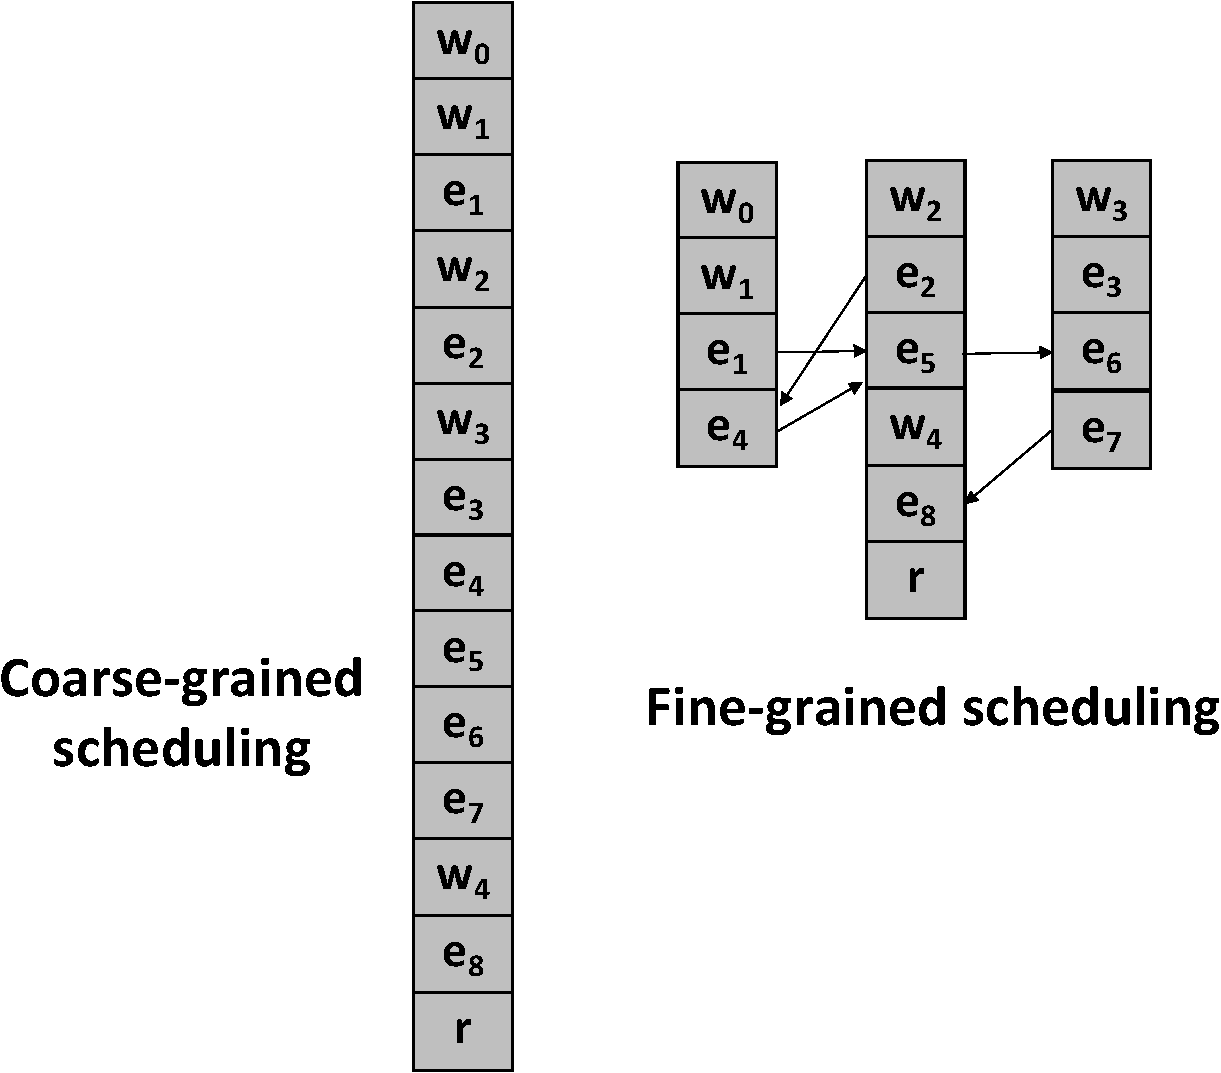
\includegraphics[scale=0.35]{Pictures/finecoarse.pdf}
		\caption{Command Queue Configurations for Scheduling \label{fig:finecoarse}}
	\end{figure}
	\par Coarse grained scheduling decisions refer to the context when all operations of kernels of a DAG are executed in its entirety first. This is achieved by setting up a single command queue on the GPU device. As a consequence, we can observe that all commands labelled by the events used in Fig. \ref{fig:motivation0} execute serially on the GPU device. In contrast if we set up multiple command queues, there is a possibility of leveraging fine grained scheduling decisions that can interleave data transfers with \textit{ndrange} operations and can execute multiple ndrange operations concurrently. In Fig. \ref{fig:finecoarse}, we setup 3 command queues for achieving this. One can observe that the writes $w_0,w_2,w_3$ can now happen simultaneously. The ndrange operations $e_1$, $e_2$ and $e_3$ can also execute concurrently on the same GPU device. However, the other commands, despite belonging to different command queues would not be able to execute simultaneously due to the precedence relationships enforced by the event dependency graph illustrated in  of Fig. \ref{fig:motivation0}.  These dependencies are represented by inter-queue edges between events in Fig. \ref{fig:finecoarse}.
	\par We note that both the cases represented in Fig. \ref{fig:finecoarse} depict one of the possible command queue configurations. In our representative example, for coarse-grained scheduling, one can have another command queue configuration where the \textit{write} command associated with $w_1$ is enqueued before that of $w_0$ or where the \textit{write} command for $w_4$ is enqueued anywhere before the \textit{ndrange} command for $e_8$. In a similar vein, one can have different command queue configurations for fine-grained scheduling as well. We next analyze how coarse-grained and fine-grained scheduling decisions for executing this DAG on a single GPU device compare with the help of the Gantt charts in Figs \ref{fig:motivation1} and \ref{fig:motivation2}. 
	\par We execute the DAG on a heterogeneous platform comprising an NVIDIA GTX-970 GPU device and a Quadcore Intel i5-4690K CPU device. The Gantt chart in Fig \ref{fig:motivation0} represents the case where a single command queue is set up for the GPU device and all the \textit{read}, \textit{write} and \textit{ndrange} commands for each of the 8 kernels are enqueued. The x-axis of the Gantt chart represents time in milliseconds (ms). The y-axis of the Gantt chart represents the kernels constituting the DAG. Each kernel is labelled with the level of the DAG to which it belongs followed by the name of the kernel operation and \textit{write}, \textit{read} and \textit{ndrange} commands pertaining to it. Each green rectangle denotes the time taken by a \textit{write} command. Each read and brown rectangle denotes the time taken by \textit{ndrange} and \textit{read} commands respectively. As evident from the corresponding Gantt chart, each command associated with each kernel executes one at a time on the GPU device resulting in an execution time of 105ms. We observe that writes occur for the first copy operation (associated with event $w0$) and for buffers of kernels in level $1$ and the kernel in level $6$. For GEMM kernels in level $1$, data is transferred for input buffers associated with events $w_1$, $w_2$ and $w_3$. Similarly for the GEMM kernel in level 6, data is transferred for the input buffer associated with event $w4$. Finally the last read associated with event $r$ occurs for the kernel in level $6$. We note that each of the operations are executed sequentially mapped to a single GPU device using a single command queue. 
	\begin{figure}[ht]  
		\centering
		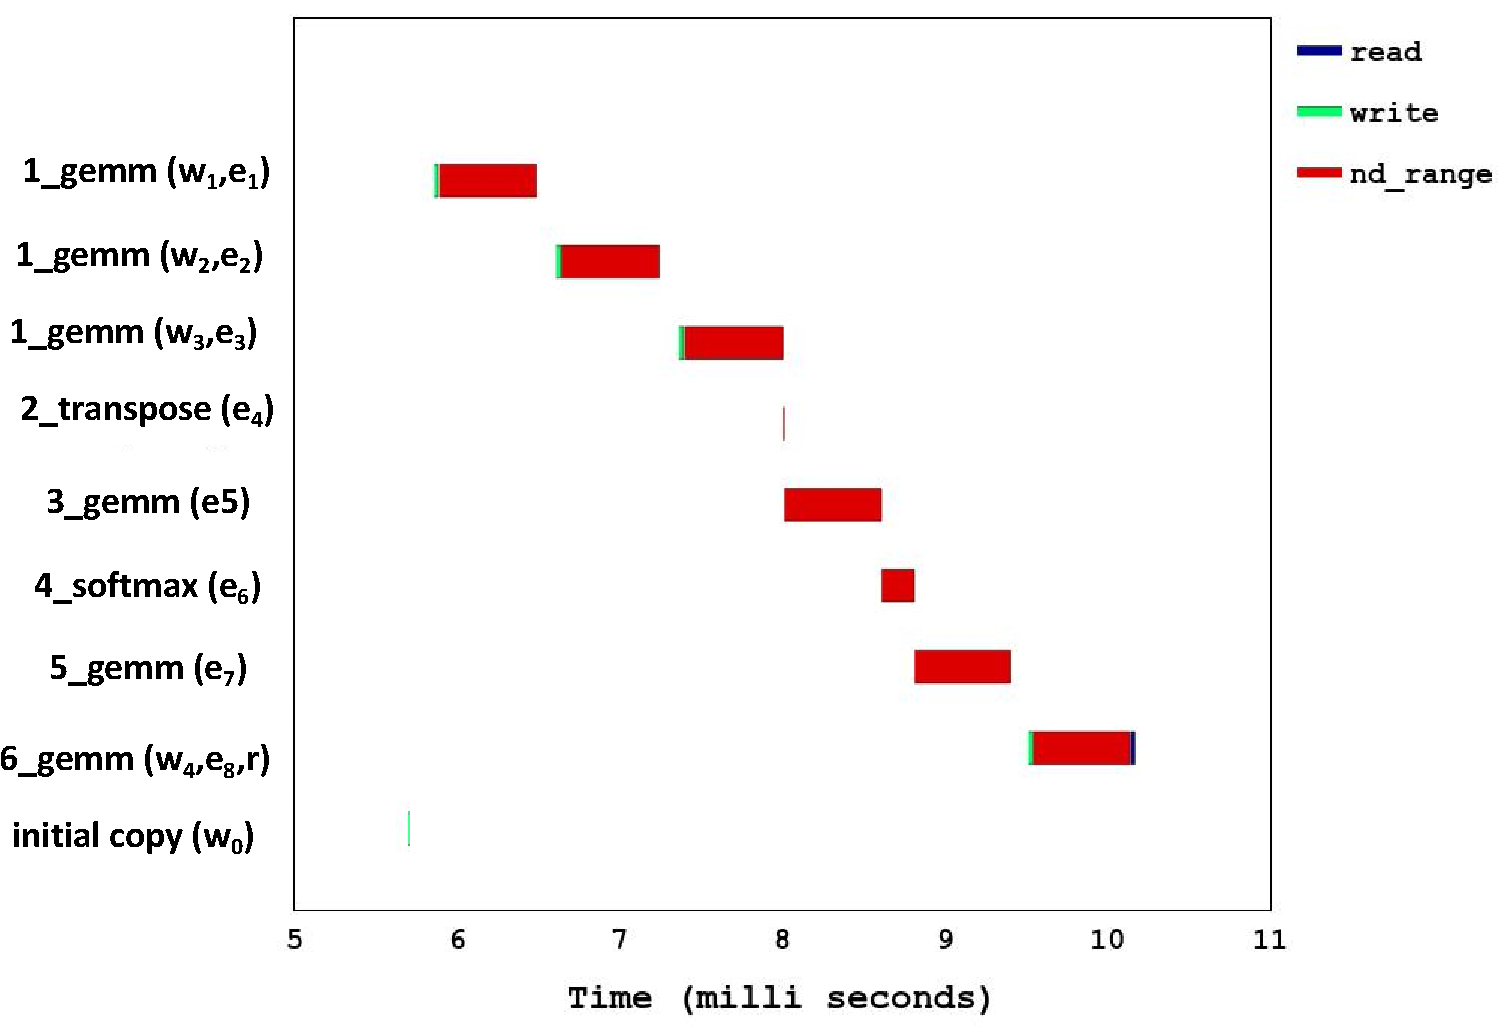
\includegraphics[scale=0.35]{Pictures/motiv_sequential.pdf}
		\caption{Sequential Execution on GPU device\label{fig:motivation1}}
	\end{figure}
	\begin{figure}[ht]  
		\centering
		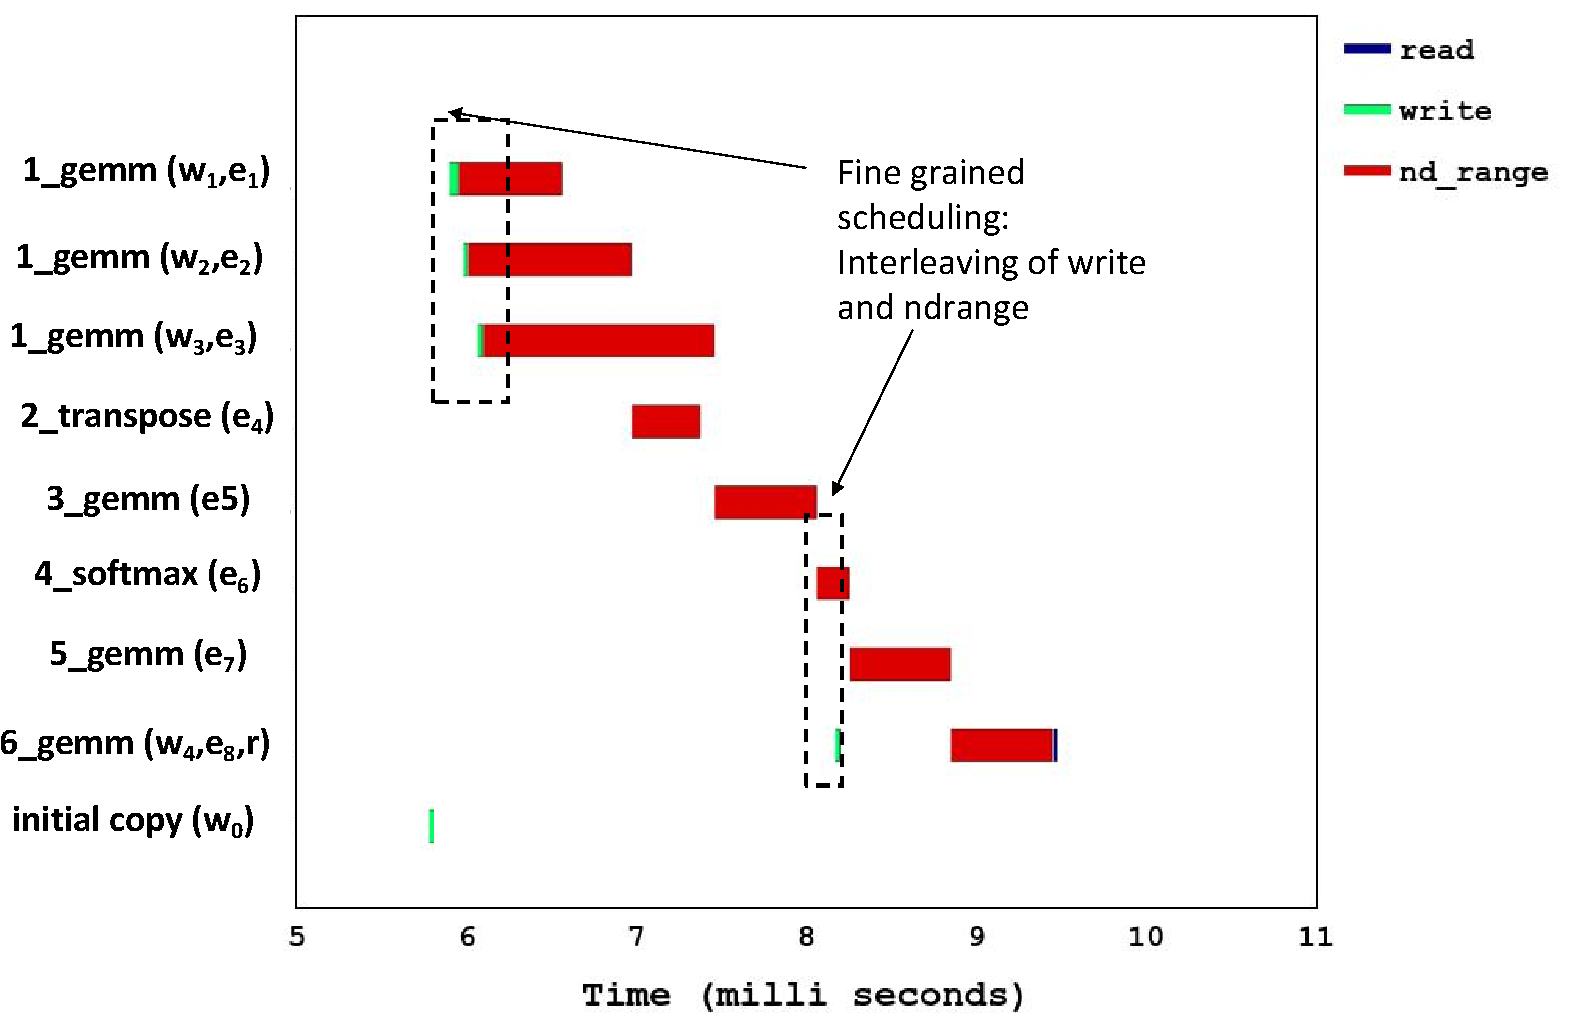
\includegraphics[scale=0.35]{Pictures/motiv_concurrent.pdf}
		\caption{Concurrent Execution on GPU device\label{fig:motivation2}}
	\end{figure}
	\par In contrast, if we set up three command queues for the same GPU device and dispatch our kernels intelligently, we observe an $8\%$ reduction in execution time , with the DAG finishing in 95ms. This reduction in time maybe attributed to the interleaving of data transfers (\textit{write} commands associated with $w1,w2$ and $w3$) with execute operations (\textit{ndrange} commands associated with events $e1,e2,e3$)  for kernels in levels $1$. It can be observed that while \textit{ndrange} command associated with $e1$ is executing, the buffer associated with $w2$ can be copied simultaneously. Similarly, $w3$ can also be copied while $e1$ and $e2$ are executing. Additionally, it can be seen that all kernels in level $1$ are  executing concurrently for the same device. It may be further observed, the individual execution times for each kernel increases slightly as a result. This is due to the fact, that different work groups of different kernels that have been concurrently dispatched  are scheduled in a round robin fashion to the compute units of the device, thus causing resource contention. However, the total time for finishing both kernels concurrently is lesser than the case when they are dispatched in sequence. We note that concurrency between three kernels and three data transfers  yields a decrease of 8 \% in execution time. In general, for one layer of the transformer a maximum of 16 such DAGs can run in parallel. In such a setting where there is more concurrency to exploit, fine grained scheduling that exploits both the CPU and the GPU devices of the heterogeneous platform by setting up multiple command queues per device shall yield more speedups.
	
	\par The typical dispatch mechanisms offered by list scheduling heuristics available in SOCL, StarPU and MultiCL are optimized for heterogeneous clusters comprising multiple devices and rely on coarse-grained scheduling decisions. They do not leverage the benefits obtained by using fine-grained scheduling decisions. We implement {\em PySchedCL} as a scheduling framework optimized for heterogeneous multicore platforms where devices support concurrent execution. Provided with the right guidance parameters by the designer, the framework shall automatically produce efficient data-parallel mapping solutions that can exploit concurrency both at the application and at the platform level.


\section{Formal Problem Statement}
\label{sec:prob}
	Let us consider a heterogeneous platform $\mathcal{P}$ depicted in Fig. \ref{fig:platprob} which comprises a CPU device and a GPU device connected via a PCI-Express bus. Each device has support for executing multiple kernels simultaneously. The OpenCL standard supports device fission for CPU devices i.e. a single CPU device can be partitioned into multiple subdevices, thereby enabling concurrent execution for the same. We consider as GPU an NVIDIA device with Hyper-Q support \cite{nvidia}. Hyper-Q offers a solution that allows the CPU host to dispatch multiple kernels simultaneously on the GPU device with the help of hardware managed work queues. 
	\par Let us represent an OpenCL application graph as a directed acyclic graph (DAG) $G = \langle K,B,E_I,E_O,E \rangle$ where $K$ denotes the set of OpenCL kernels, $B= B_I \bigcup B_O$ represents the set of buffers for all $k \in K$. The set $B_I$ denotes the set  of input buffers and the set $B_O$ denotes the set of output buffers. The set $E_I \subseteq B_I \times K$ denotes the set of edge dependencies between each input buffer and kernel, $E_O \subseteq K \times B_O$ denotes the set of edge dependencies between each kernel and output buffer. The set $E \subseteq B_O \times B_I$ denotes the set of input output buffer dependencies across kernels in the DAG. Command queues are typically setup per device depending on which kernels are mapped to which devices. 
	\begin{figure}[ht]
		\centering
		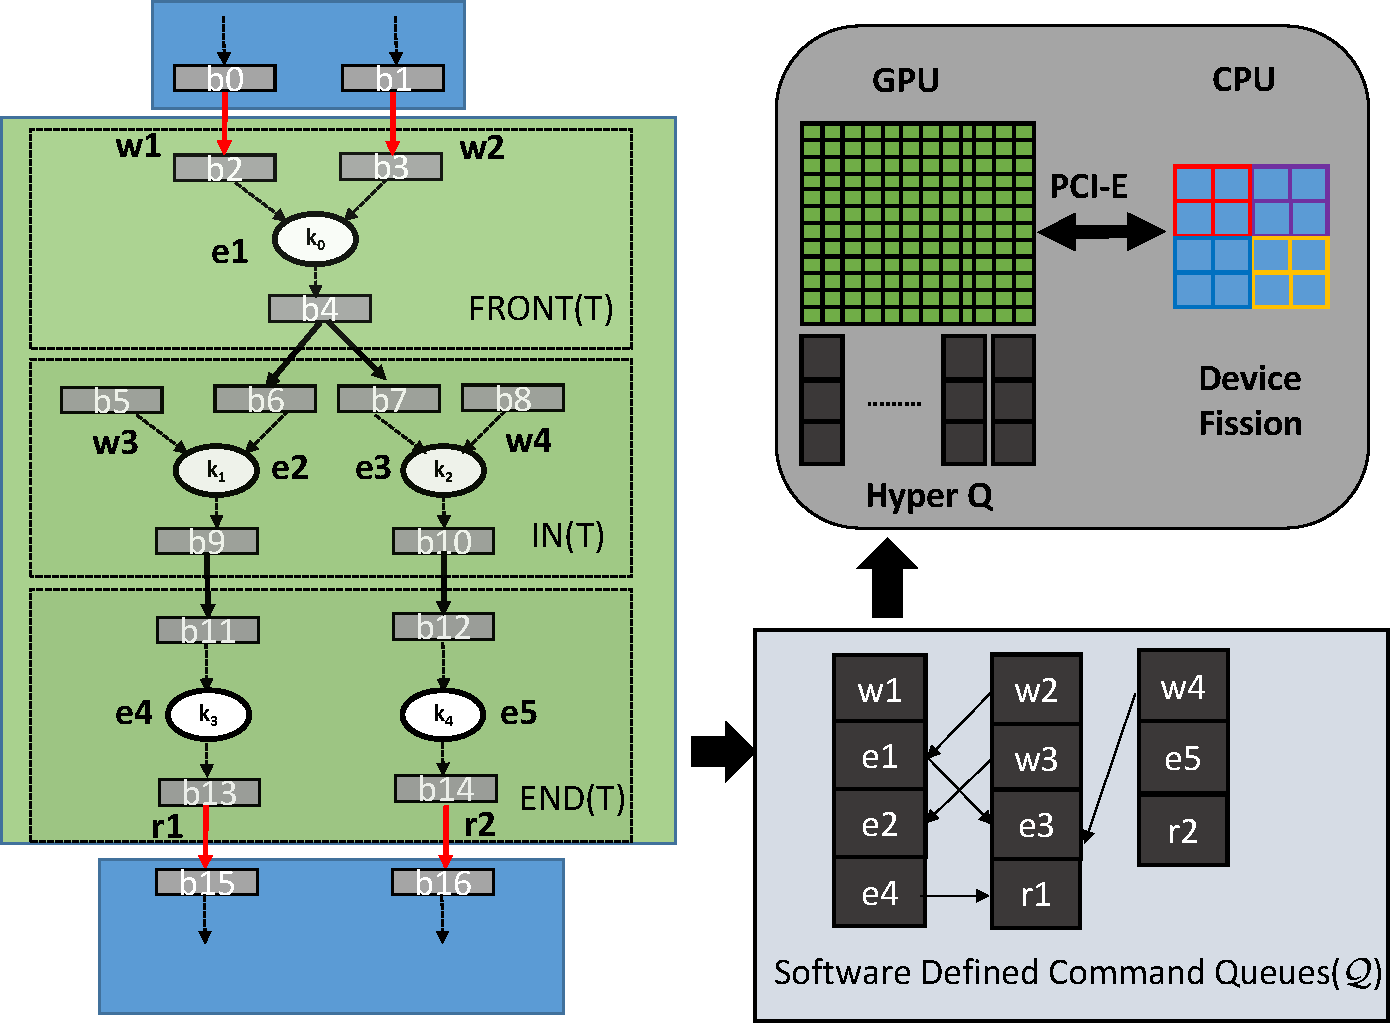
\includegraphics[scale=0.38]{Pictures/PlatformAndProblemFormulation.pdf}
		\caption{\small Platform and DAG Model\label{fig:platprob}}
	\end{figure}
	
	\begin{definition} \label{def:task-component}
		\emph{Given an OpenCL DAG $G=\langle K,B,E_I,E_O,E \rangle$, we denote a task component $T_d$ as a subset of kernels $K^\prime \subseteq K$  where each kernel $k$ is mapped to the same device $d$.} 
	\end{definition}

	\par In our case, $d= \{ cpu,gpu \}$. In Fig. \ref{fig:platprob}, we have $T_{gpu} = \{k_0,k_1,k_2,k_3,k_4 \}$. For a given task component we define the following terminology.
	\begin{definition}
		\emph{Given a task component $T_d$ pertaining to some OpenCL DAG $G$, we define $FRONT(T_d)$ as the set of kernels where each kernel $k$ has input buffer dependencies $(b_i,k) \in E_I$ such that for $b_i$, if there exists an immediate predecessor $b_j$ where $(b_j,b_i)\in E$ and $(k^\prime,b_j) \in E_O$, then the kernel $k^\prime$ belongs to a different task component $T^\prime_{d'}$.} 
	\end{definition}
	In Fig. \ref{fig:platprob}, we observe that $FRONT(T) = \{ k_0\}$, since both input buffers $b2$ and $b3$ have predecessors pertaining to kernels belonging in a different task component. 
	\begin{definition}\emph{
		Given a task component $T$ pertaining to some OpenCL DAG $G$, we define $END(T)$ as the set of kernels where each kernel $k$ has output buffer dependencies ($k,b_i) \in E_O$ such that for $b_i$ if there exists an immediate successor $b_j$ where $(b_i,b_j)\in E$ and $(b_j,k^\prime) \in E_I$ then kernel $k^\prime$ belongs to a different task component $T^\prime_{d'}$.}
	\end{definition}
	In Fig. \ref{fig:platprob}, we can observe that $END(T_{gpu})=\{k_3,k_4\}$, since both output buffers $b13$ and $b14$ are used as inputs for kernels belonging to a different task component.
	\begin{definition}\emph{
		Given a task component $T_d$ pertaining to some OpenCL DAG $G$, we define $IN(T)$ as the set of kernels where each kernel $k \in T_d, k \notin FRONT(T), k \notin END(T)$. } 
	\end{definition}
	In Fig. \ref{fig:platprob}, we can observe that $IN(T)=\{k_1, k_2 \}$
	
	We classify buffer edge dependencies $(b_i,b_j) \in E$ into two categories -i) intra-edge, ii) inter-edge.
	\begin{definition}\emph{
		Given a task component $T_d$ pertaining to a DAG $G$, an edge $(b_i,b_j)$ is said to be intra-edge if there exists kernels $k_i,k_j$ such that $(k_i,b_i) \in E_O$, $(b_j,k_j) \in E_I$ and both kernels $k_i,k_j$ belong to the same component.} 
	\end{definition}
	In Fig. \ref{fig:platprob}, we can observe that $(b4,b6)$ and $(b4,b7)$ are intra-edges for $T_{gpu}$.
	\begin{definition}\emph{
		Given two task components $T_x$ and $T_y$ pertaining to a DAG $G$, an edge $(b_i,b_j)$ is said to be an inter-edge from $T_x$ to $T_y$ if there exists kernels $k_i,k_j$ such that $(k_i,b_i) \in E_O$, $(b_j,k_j) \in E_I$ and kernel $k_i$ belongs to $T_x$ and $k_j$ belongs to $T_y$.}
	\end{definition}
	In Fig. \ref{fig:platprob}, we can observe that $(b0,b2)$, $(b1,b3)$, $(b13,b15)$ and $(b15,b16)$ are inter-edges.
	We classify kernel-buffer dependencies in $E_I$ and $E_O$ into two categories - i) isolated copy and ii) dependent copy
	\begin{definition}\emph{
		Given any kernel $k_i$, an edge ($b_i,k_i)\in E_I$ represents an isolated copy (write) {\em iff} for every $b_k \in B$, $(b_k,b_i) \notin E$.
		In a similar fashion, an edge ($k_i,b_j)$ represents an isolated copy(read) {\em iff} for every $b_k \in B$, $(b_j,b_k) \notin E$ respectively.}
	\end{definition}
	In Fig. \ref{fig:platprob}, the edges $(b5,k_1)$ and $(b8,k_2)$ correspond to isolated writes. 
	\begin{definition}\emph{
		Given any kernel $k_i$ pertaining to a task component $T_d$, an edge ($b_i,k_i)\in E_I$ represents a dependent copy (write) {\em iff} there exists some buffer $b_i \in B$ such that  $(b_i,b_k)\in E$.
		In a similar fashion, an edge ($k_i,b_i$) represents a dependent copy(read) {\em iff} there exists some $b_k \in B$ such that $(b_j,b_k) \in E$.} 
	\end{definition}
	In Fig. \ref{fig:platprob}, every buffer-kernel dependency apart from $(b5,k_1)$ and $(b8,k_2)$ correspond to dependent copies.
	\begin{definition}\emph{
		Given a task component $T_d$ of an application DAG $G$ mapped to a device $d$ with $r$ command queues, we define the command queue data structure $\mathcal{Q}$ as a graph $\langle V_Q, E_Q\rangle$  where $V_Q=\{q_1,q_2,\cdots,q_r\}$ denotes the set of command queues allocated to $T_d$. Each element $o_i$ belonging to each queue $q_i$ constitutes either a \textit{write}, \textit{ndrange} or \textit{read} operation pertaining to some kernel belonging to $T_d$. Each element of the set $E_Q$ is an edge of the form $\langle o_i,o_j \rangle$ where  $o_i \in q_r$ and $o_j \in q_s$ such that  $q_r \neq q_s$ and represents the precedence constraints enforced by the edges in the DAG $G$. }
	\end{definition}
	The framework uses an $enq$ procedure that sets up the data structure $\mathcal{Q}$ for task component $T_d$ as follows.
	An operation $o_i$ pertaining to kernel $k_i$  is enqueued to one of the command queues in $V_Q$ depending upon the membership of $k_i$ in the sets $IN(T_d)$, $FRONT(T_d)$ and $END(T_d)$. This is described below.
	\par \noindent i)If $k_i \in FRONT(T_d)$, the enqueue procedure $enq$ enqueues all dependent write commands for buffers $b_j$ corresponding to dependent writes $(b_j,k_i) \in E_I$ followed by the ndrange command for $k_i$.
	\par \noindent ii) If $k_i \in END(T_d)$, the enqueue procedure $enq$ enqueues the ndrange command for $k_i$ followed by all dependent read commands for buffers $b_j$ corresponding to intra-edges $k_i,b_j \in E_O$.  
	\par \noindent iii) If $k_i \in IN(T_d)$, the enqueue procedure $enq$ enqueues only the ndrange command for $k_i$ 
	\par \noindent iv) For every kernel $k_i$  belonging to $FRONT(T)$, $IN(T) $and $END(T)$, the enqueue procedure $enq$ enqueues all isolated writes for input buffers $b_j$, $(b_j,k_i) \in E_I$ before enqueuing the ndrange command for $k_i$ and all isolated reads for output buffers $b_r$, $(k_i,b_r) \in E_O$ after enqueueing the ndrange command for $k_i$. 
	\par An edge $(o_i,o_j) \in E_Q$ exists if i) $o_i$ is a isolated/dependent write $(b_r,k_s)$ and $o_j$ is an ndrange operation for kernel $k_s$ ii) $o_i$ is an ndrange operation for kernel $k_s$ and $o_s$ is a dependent/isolated write $(k_s,b_r)$ and iii)both $o_i$ and $o_j$ are ndrange operations for kernels $k_r$ and $k_s$ respectively such that there exists edges $(k_r,b_r) \in E_O$, $(b_s,k_s) \in E_I$  and $(b_r,b_s) \in E$ is an intra edge. In Fig. \ref{fig:platprob}, $(b_3,k_0)$ corresponds to a dependent write for kernel $k_0$ thus requiring a dependency between associated operations $w_2$ and $e_1$ in $\mathcal{Q}$.  The edge $(e_1,e_3)$ represents the dependency between kernels $k_0$ and $k_2$ arising due to the dependencies $(k_0,b_4)$,$(b4_b7)$,$(b_7,k_2)$ where $b_4,b_7$ is an inter edge. 
	\par The framework expects that the device preferences for each kernel are known beforehand. Using this information and the $enq$ procedure, the framework can emulate dynamic coarse-grained scheduling decisions supported by frameworks like StarPU and SOCL where kernels are dispatched one at a time to devices. For fine-grained scheduling algorithms it is expected that the user provides an initial decomposition of the DAG $G$ into a set of task components $\mathcal{T}$ where each task component $T_d \in \mathcal{T} \in \mathcal{T} $ is mapped to a particular device $d$. Additionally, one must provide as guidance parameters for each task component $T_d$, the number of command queues to be used. Given this as input, the framework automatically sets up multiple command queues inside each task component for  device $d$ and outputs a schedule $\sigma$ which is an ordered sequence of $enq$ procedures that respects the precedence relationships of the application DAG. The problem formulation is formally stated as follows.
	\begin{definition}\emph{
		Given a DAG $G = \langle K,B,E_I,E_O,E \rangle$,  a corresponding set of $m$ task components $\mathcal{T} = \lbrace T_{d_1}, T_{d_2}, \cdots, T_{d_p}\rbrace$ and a target heterogeneous CPU-GPU multicore platform $\mathcal{P} = \{d_1,d_2,\cdots d_p \}$ containing $p$ devices, a schedule $\sigma$ is an ordered sequence of enqueue procedures $enq(T_{d_1}), enq(T_{d_2}),\cdots,enq(T_{d_p})$ such that the kernels $k_i \in K$ is dispatched in a topologically sorted fashion i.e sorted with respect to the ordering of $k_i$'s enforced by the edges in $G$,  $k_1 \preceq k_2 \preceq \cdots, k_{|K|}$. } 
	\end{definition}
	 
% Chapter Template

\chapter{Software Architecture} % Main chapter title

\label{Chapter4} % Change X to a consecutive number; for referencing this chapter elsewhere, use \ref{ChapterX}

\lhead{Chapter 4. \emph{Software Architecture}} % Change X to a consecutive number; this is for the header on each page - perhaps a shortened title

An overview of the software architecture for {\em PySchedCL} is depicted in Fig. \ref{fig:pyschedcl}. The framework consists of two distinct modules, the functionalities of which are elaborated as follows.
	\begin{figure}[ht]  
		\centering
		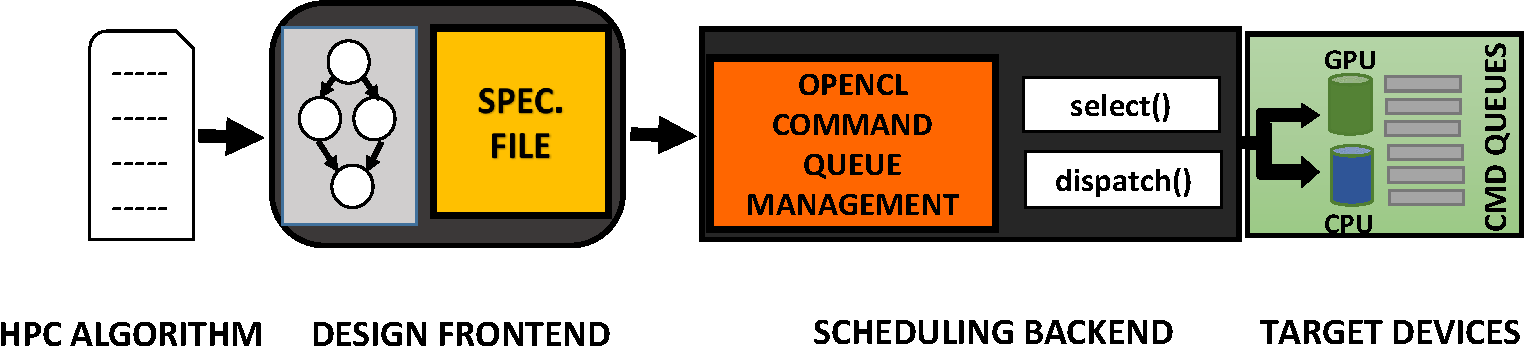
\includegraphics[scale=0.35]{Pictures/TCOverviewNonML.pdf}
		\caption{PySchedCL Toolflow\label{fig:pyschedcl}}
	\end{figure}
	\begin{enumerate}
		\item \textbf{Design Frontend: }The input to the scheduling framework is an OpenCL application represented in the form of a task graph $G$ as discussed earlier. The proposed framework supports a specification file using which programmers can easily design an OpenCL application for execution on a heterogeneous platform. The programmer requires to implement only the OpenCL kernels and provide configuration parameters  such as the dimensions of the input/output dataspace along with dependency information between kernels in this specification file.
		\item \textbf{Scheduling Backend: }The scheduling backend takes as input the specification file in Step 1, and schedules the computation of each data parallel kernel in the application across the devices of a heterogeneous CPU/GPU platform. This is achieved with the help of select and dispatch routines. The framework uses the {\tt select} function to i)choose a task component from $G$ and ii) select an available device (CPU/GPU). It next uses the {\tt dispatch} (line 8) routine for finally issuing relevant write, ndrange and read commands now specified in $\mathcal{Q}$ to target devices. The backend API also supports end designers to implement custom scheduling heuristics by overriding the functionalities of the {\tt select} and {\tt dispatch} routines.
		%In this communication, we highlight how popular scheduling heuristics such as standard list scheduling policies \cite{heft,zhao1,zhao2,hcpt,hps,pets,lookahead,plannerguide,owm,fdws} as well as standard cluster scheduling policies \cite{triplet,chp,rac,fcs,cmwsl} can be implemented. We also show how statistics obtained statically for a target application can be used along with the scheduling policies for designing intelligent scheduling heuristics. 
	\end{enumerate}
    The modular design of the scheduling backend is an integral feature of the framework. The default {\tt select} routine expects a static assignment of kernels to devices prior to the execution. It can be substituted by the user very easily with other scheduling policies which can even be dynamic in nature. The experimental section of this thesis extensively uses this modular feature of the {\tt select} function to implement and compare several scheduling policies on the transformer DAG. Additionally, experiments with a Machine Learning based scheduling policy have also been performed in a similar fashion. 
    \par We next elicit implementation details for each of the two modules  constituting the framework in the following subsections. 
    
    \section{Input File Specification}
	The specification file used in {\em PySchedCL} is written using the Javascript Object Notation (JSON) file format. The file consists of a collection of key value pairs depicting  necessary attribute information for an OpenCL kernel which includes information regarding input/output buffers, variables passed as arguments to the kernel call, the dimension of the kernel etc. Our tool processes this specification file and uses the scheduling backend to mimic the execution of a host program executing this kernel. 
	\par We have a LLVM compiler pass which parses the abstract syntax tree of an OpenCL kernel and generates an incomplete JSON file. The pass understands the dimensionality of the kernel, the types and positions of each variable and buffer used in the kernel function call. It also classifies buffers as input/output buffers by understanding whether it is treated as \textit{l-values} or \textit{r-values} in the body of the function. Given this file, the user is only required to specify guidance parameters which include -i) the size of the buffers ii) the number of work items iii) the values of the variable arguments and iv) the device and the number of command queues to be used. The user has the option of either hardcoding constant numbers or writing expressions containing symbolic variables that depicts the relationship between work items and the dataspace to be processed. This ensures that we have one specification file for a kernel and the final values of these symbolic variables can be provided as command line parameters at runtime. We explain this by designing a JSON specification file for the matrix multiplication kernel depicted in Listing 1.

    \begin{lstlisting}[caption={OpenCL Kernel for Matrix Multiplication},captionpos=b,frame=single,basicstyle=\tiny,language=C]
        __kernel void gemm(__global float *A, __global float *B, __global float *C, 
        int M, int N, int K) {
        int ty = get_global_id(1);
        int tx = get_global_id(0);
        if ((tx < N) && (ty < M))
        {
        C[ty * N + tx] = 0;
        for(int k=0; k < K; k++)
        C[ty * N + tx] += A[ty * K + k] * B[k * N +tx];
        }
        
        }
    \end{lstlisting}

    The matrix multiplication kernel is a 2-D kernel which takes as input two matrices $A$, $B$ of dimensions $M \times K$, $K \times N$ respectively and produces an output matrix $C$ of dimension $M \times N$. A total of $M*N$ work items is launched where the job of each work item is computing the dot product of one row of $A$ and one column of $B$ to produce one element of $C$. The JSON specification file for the same is depicted in Fig. \ref{fig:json}
    
    \begin{figure}[ht]  
		\centering
		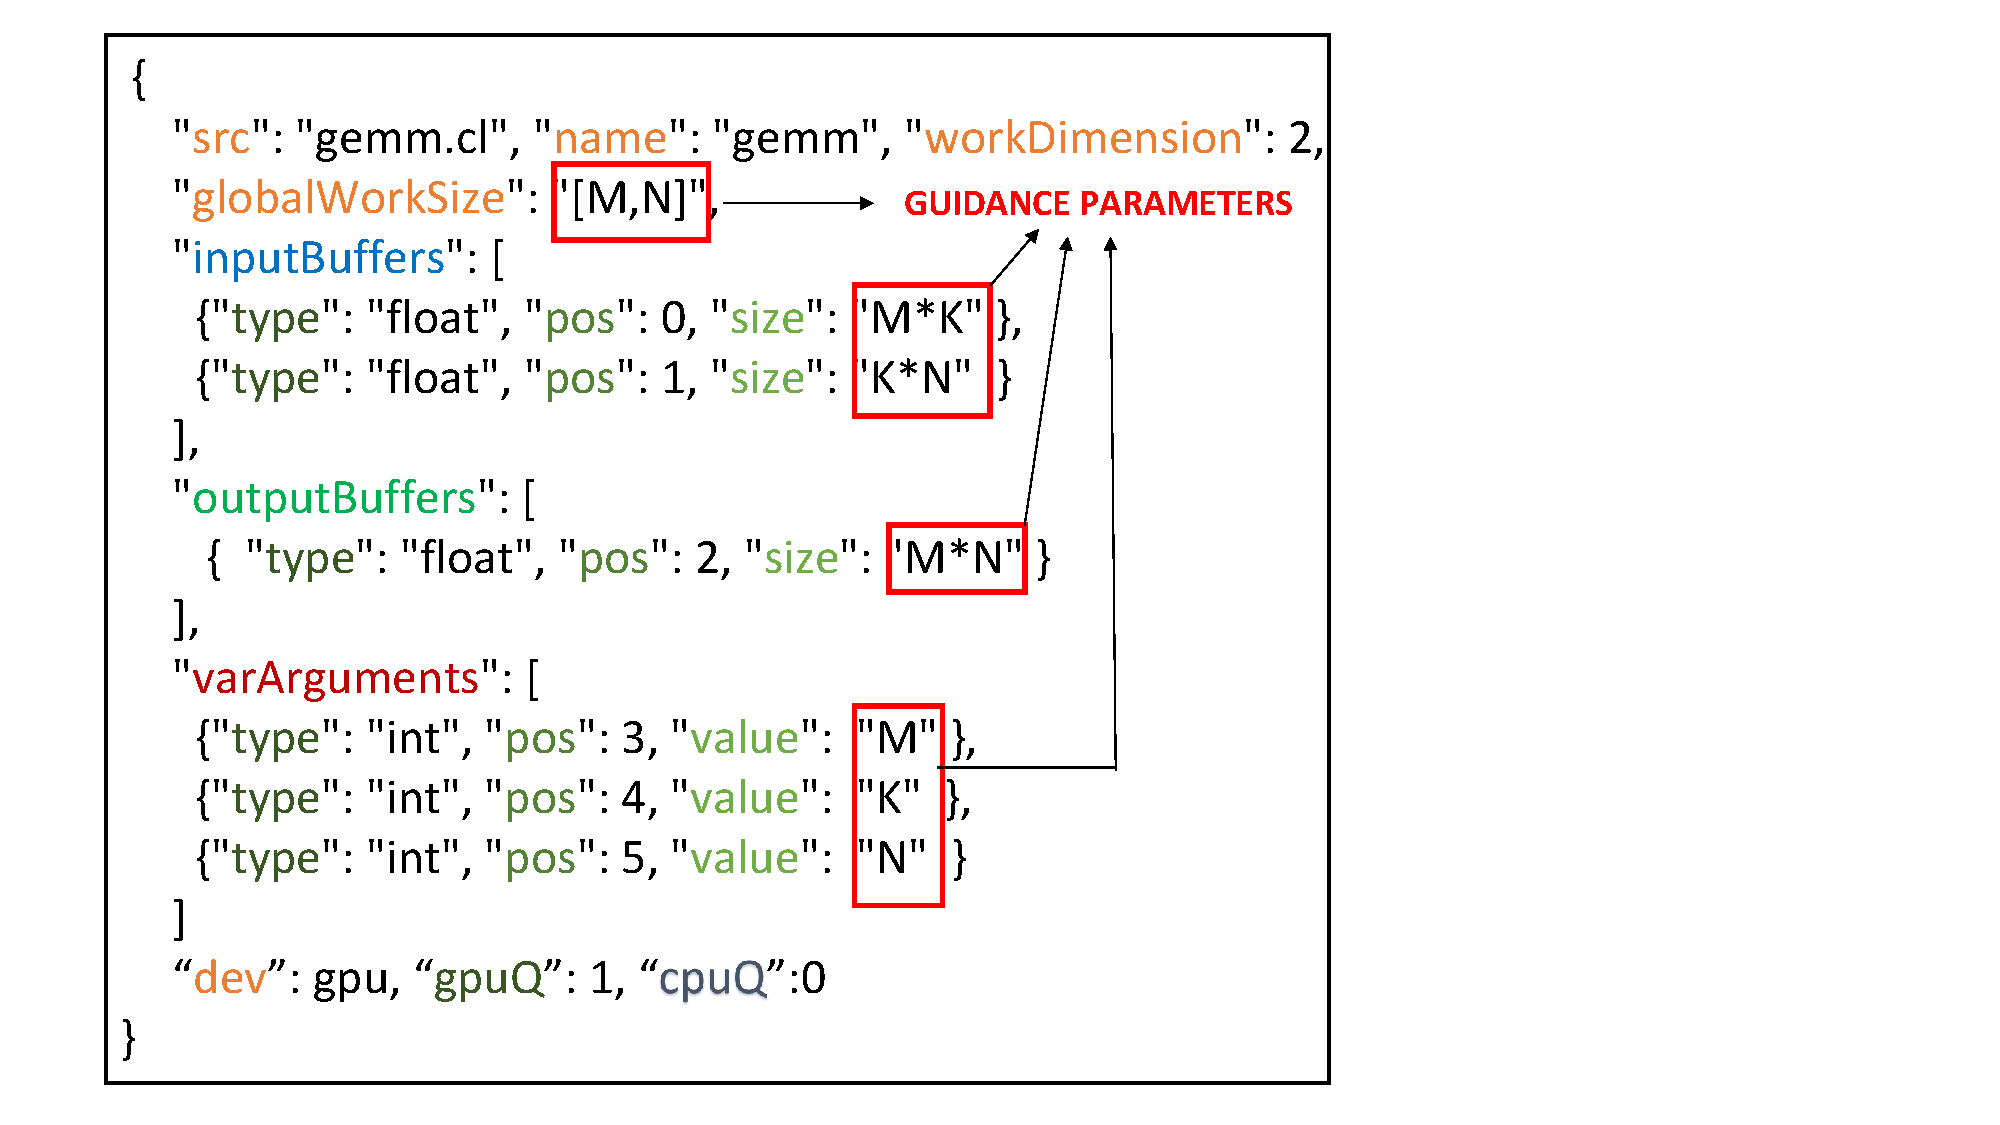
\includegraphics[scale=0.4]{Pictures/json_file.pdf}
		\caption{JSON File for Matrix Multiplication \label{fig:json}}
    \end{figure}
    
    The file comprises the following information.
	\begin{enumerate}
		\item \textbf{Kernel Information: } This includes i) the name of the OpenCL kernel function (which is {\tt gemm} in Fig. \ref{fig:json}), ii) the filepath of the required kernel source file, iii) the dimensionality of the kernel in {\tt workDimension} and iv) the total number of work items ({\tt globalWorkSize}) to be launched for this kernel. The variable {\tt globalWorkSize} is a three element list where each element refers to the number of work items along a particular dimension. As guidance parameters, the user can specify these elements either as compile time constants or using an generic expression containing symbolic variables. For the example JSON file, we have {\tt globalWorkSize = [M,N,1]}. The values of $M$ and $N$ can be configured  as command line parameters right before dispatching the kernel.  
		\item  \textbf{Buffer Information: }  The JSON file maintains information for three buffer lists - {\tt inputBuffers} reserved for input buffers, {\tt outputBuffers} reserved for output buffers and {\tt ioBuffers} reserved for buffers which are treated as both input and output  by the kernel. Each buffer belonging to any one of the lists is characterized by the tuple $\langle type, size ,pos \rangle$ where $type$ denotes the data type for each element in the buffer, $size$ denotes the total number of elements in the buffer, and $pos$ denotes the index position of the buffer argument in the actual function call of the kernel. For example, the input buffer passed as argument in the first position of the function call in Listing 1 has  $pos=0$. The user can configure the guidance parameter $size$ for each buffer either as a compile time constant or an expression of symbolic variables. For the example JSON file in Fig. \ref{fig:json}, the sizes of the buffers are the number of elements for each matrix. 
		\item \textbf{Kernel Arguments: } In the JSON file, each variable argument passed as an argument to the OpenCL function call is denoted by the tuple $\langle type, value, pos\rangle$  where $type$ denotes the type of the variable, $value$ represents the value contained in the variable and $pos$ represents the index position of the variable argument in the actual function call of the kernel. The user can configure the guidance parameter $value$  again either as a compile time constant or as a symbolic variable. In Fig. \ref{fig:json}, we have three variable arguments $M,N,K$ each depicting the size of one dimension of the matrices.
		\item \textbf{Device Information: } Finally, the $dev$ field indicates which device to be used. The fields $gpuQ$ and $cpuQ$ denote the number of command queues to be used for the GPU and the CPU devices respectively.
    \end{enumerate}
    
    \begin{figure}[ht]
		\centering
		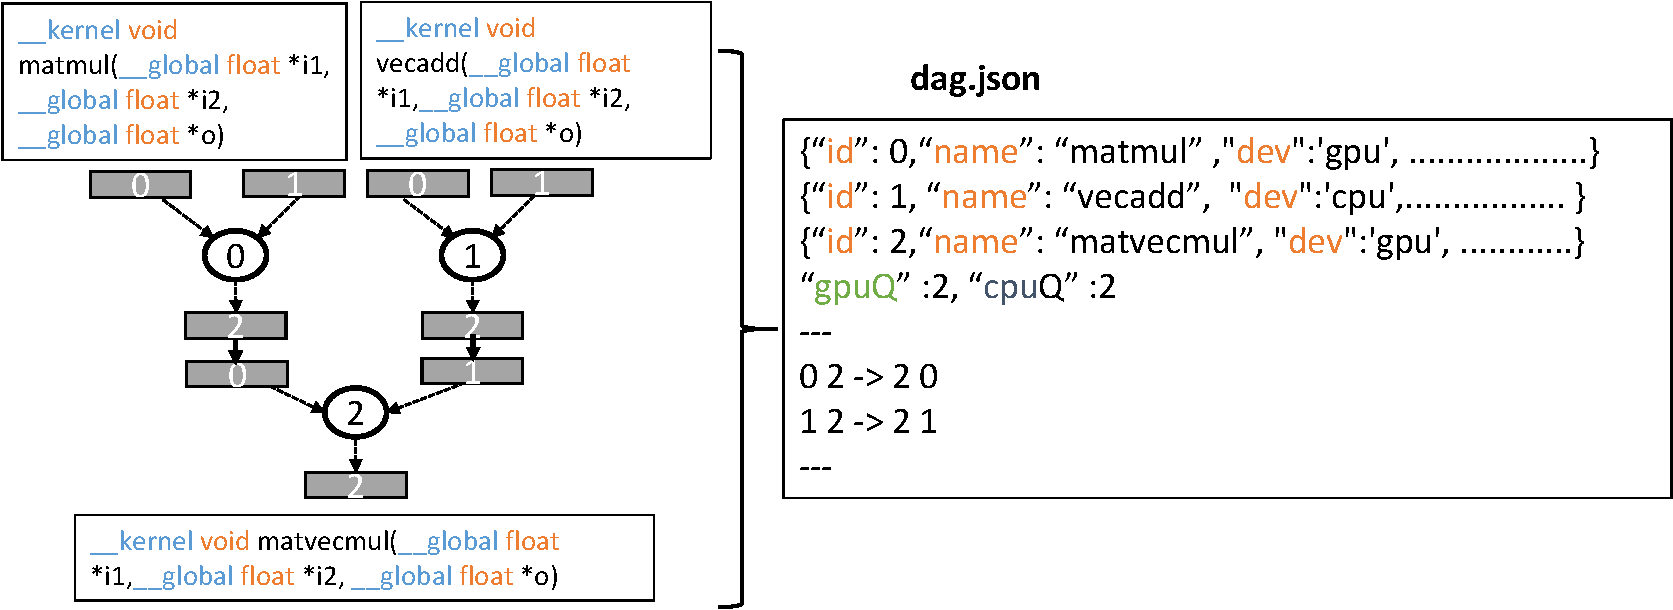
\includegraphics[scale=0.5]{Pictures/DAGJson.pdf}
		\caption{\small OpenCL DAG Specification\label{fig:OpenCLDAG}}
	\end{figure}
	\par \noindent In general a DAG of OpenCL kernels, can be specified as a single JSON file which contains the information regarding each kernel generated by running the compiler pass on each kernel. The user additionally has to specify information that captures the precedence constraints of the DAG. Unlike frameworks like SOCL, StarPU and MultiCL which requires implementing host-side implementations, our framework relies only on the DAG specification provided as a simple JSON file with configuration parameters of individual kernels and dependency information of the DAG.  
    \par Let us consider an example DAG comprising three kernels as depicted in Fig. \ref{fig:OpenCLDAG}. Each kernel now is designated by a unique identifier field called $id$. The kernel with id $0$ represents matrix multiplication kernel which takes as input two matrices of dimensions $M \times K$ and $K \times N$ and produces an output of dimension $M \times N$. The corresponding sizes of the input and output buffers are specified inside the JSON file of the kernel using these symbolic variables. The kernel with id $1$ represents a vector addition kernel which takes two vectors of size $N$ and produces one output vector of size $N$. The kernel with id $2$ represents  matrix-matrix multiplication kernel which takes as input an $M\times N$ matrix and $N\times 1$ vector and produces an $M \times 1$ vector. Again, the corresponding sizes of the input and output buffers for these kernels are specified in the individual JSON files of the kernels. The outputs of the kernels $1$ and $2$ are used by the kernel with id $2$. The dependency information for the same is specified as a set of edges of the form $k_i,b_r \rightarrow k_j,b_s$, where $k_i$,$k_j$ represent kernel ids that are dependent, $b_r$ is an output buffer of $k_i$ and $b_s$ is an input buffer of $k_j$ i.e. $(k_i,b_r) \in E_O$, $(b_s,k_j) \in E_I$ and $b_r,b_s \in E$. The ids for the buffers $b_r$ and $b_s$ are represented by their corresponding argument positions in the function call for the kernels. For example, if we consider $0,2 \rightarrow 2, 0$, the output buffer specified in argument 2 of kernel $0$ will be used as input buffer specified in argument 0 of kernel $2$. As guidance parameters, the user can specify the device preference for each kernel using the {\tt dev} field. In Fig. \ref{fig:json}, the kernels with ids 0 and 2 are mapped as a task component to the GPU device while kernel with id $1$ is mapped to the CPU device. The framework automatically takes care of setting up command queues specified in the fields $cpuQ$ and $gpuQ$ so as to maximally exploit concurrency using the scheduling engine which is discussed next.
    
    \section{Scheduling Backend}
    An overview of the scheduling backend is depicted in Fig. \ref{fig:schedbackend}. We explain the working principle of the backend with the help of the procedure $schedule$ highlighted in Algorithm \ref{algo:dispatch} for scheduling. The input to $schedule$ is the application graph $G$ and the set of devices in the target platform $\mathcal{P}$. The procedure first parses the input specification and extracts the set of task components that are ready for dispatch (line 2).

    \begin{definition}
        \emph{We say a task component $T$ is \textbf{ready for dispatch} if for any kernel $k_i \in FRONT(T)$, i) there exists no predecessor or ii) all predecessors of $k_i$ have finished execution.}
    \end{definition} 

    \begin{algorithm}[H]
		
		\caption{Scheduling in PySchedCL\label{algo:dispatch}}
		\textbf{Input: } $G$ - an OpenCL Application DAG, $\mathcal{P}$ - set of target platform devices
		\begin{algorithmic}[1]
			\Procedure{schedule}{$G$,$\mathcal{P}$}
			\State $\mathcal{F} \leftarrow get\_free\_task\_components(G)$ , $\mathcal{A} \leftarrow \mathcal{P}$
			\While{all kernels of $G$ not finished}
			\While{$\mathcal{A}$ contains a device and $\mathcal{F}$ is not empty}
			\State $T,Q \leftarrow select(\mathcal{F},\mathcal{A})$
			\State $enq(T,Q)$
			\State $set\_callbacks(T,Q)$
			\State $dispatch(T,Q)$
			\EndWhile
			\EndWhile
			\EndProcedure
			\Function{enq}{$T_d$,$\mathcal{Q}$} 
			\State free\_kernels $\leftarrow get\_ready(T_d)$
			\While{all kernels of $T_d$ not processed}		
			\State $k \leftarrow free\_kernels$
			\State $q \leftarrow pop(\mathcal{Q})$
			\State $enqueue(k,q)$
			\State $set\_dependencies(k,\mathcal{Q})$
			\State $push(q,\mathcal{Q})$
			\State $update\_processed(free\_kernels)$
			\EndWhile
			\EndFunction
		\end{algorithmic}
	\end{algorithm}

    
   
    Each such task component is pushed into the centralized task queue $\mathcal{F}$ for dispatch. We note that task components can be individual kernels or a collection of kernels as specified by the guidance parameters in the specification file. For the former case, the decisions are coarse-grained in nature i.e. all the operations associated with a kernel $k_i$ are finished before proceeding to execute a successor kernel $k_j$.
    The set $\mathcal{A}$ represents the set of available devices and is initialized to all the devices contained in $\mathcal{P}$. The procedure $schedule$ operates on tasks belonging to the task queue $\mathcal{F}$ by selecting and dispatching free task components whenever there exists an available device in $\mathcal{A}$ (lines 4-8). This is continued until all kernels of the DAG have been processed (line 3). The $select$ routine is used to select a task component $T$ and an empty command queue data structure $\mathcal{Q}$ for an available device belonging to $\mathcal{A}$. The number of command queues to be used in $\mathcal{Q}_d$ for a device $d$ is specified as a guidance parameter by the user in the specification file. 
	\begin{figure}[ht]
		\centering
		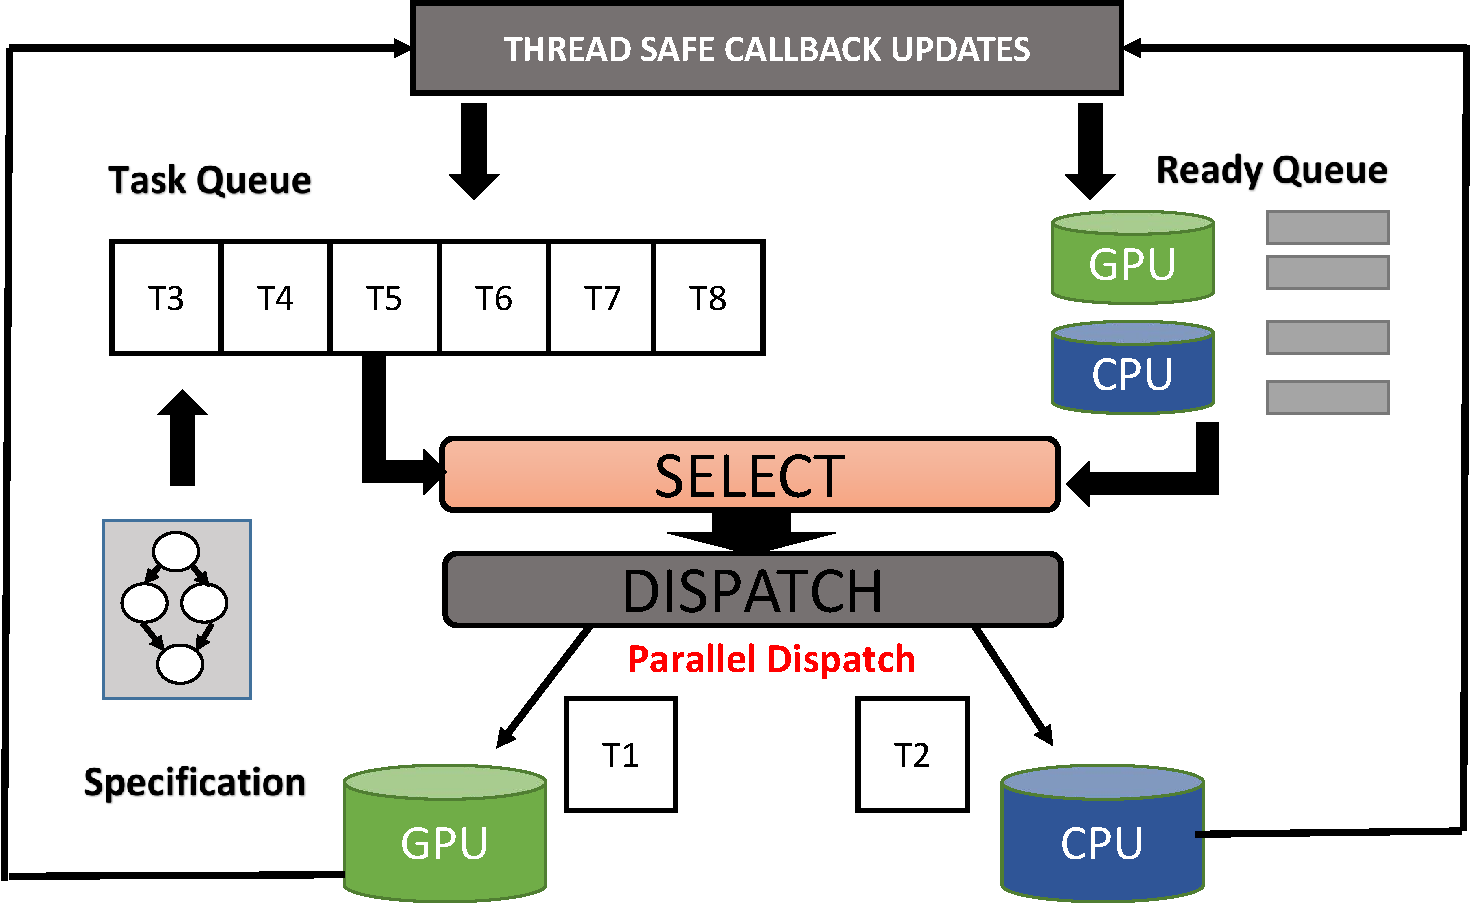
\includegraphics[scale=0.35]{Pictures/SchedulingEngine.pdf}
		\caption{\small Command Queue Setup\label{fig:schedbackend}}
    \end{figure}
    
    Given any task component $T_d$ and the empty command queue data structure $\mathcal{Q}$ for a device $d$, the $enq$ procedure is used to populate  $\mathcal{Q}$ with operations pertaining to kernels belonging to $T_d$ as discussed in Section \ref{sec:prob}.  We explain the working principle of the function with the help of an illustrative example depicted in Fig. \ref{fig:dispatch} where we map a task component comprising 5 kernels to a GPU device using a total of 3 command queues. 
	\begin{figure}[ht]
		\centering
		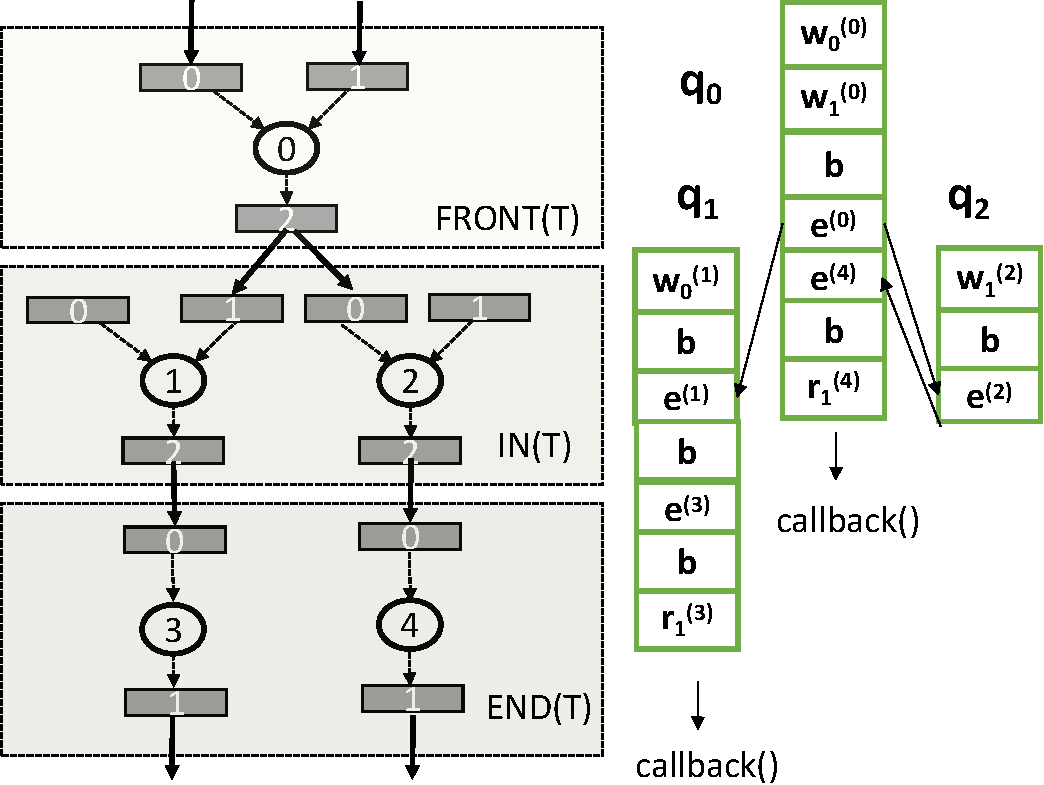
\includegraphics[scale=0.45]{Pictures/TaskObject.pdf}
		\caption{\small Command Queue Setup\label{fig:dispatch}}
	\end{figure}
	Given the task component, the function first identifies the set of free kernels ready for dispatch and stores them in the list $ready\_kernels$. (line 10). A free kernel of a task component represents either a kernels in $FRONT(T)$ or a kernel whose predecessors have been processed for setting up $\mathcal{Q}$. A free kernel $k$ is first selected from $ready\_kernels$ (line 10) and a queue $q$ is selected from $V_Q$ of $\mathcal{Q}$ using $pop(\mathcal{Q})$(line 5). The list of command queues $V_Q$ in $\mathcal{Q}$ is maintained as a circular queue by the framework. The required read,write and ndrange operations of kernel $k$ are next pushed to command queue $q \in V_Q$. In Fig. \ref{fig:dispatch}, we observe for kernel $0$, two write operations $w_0^{(0)},w_1^{(0)}$ being pushed first to $q_0$ followed by a barrier, and an ndrange operation $e^{0}$. Since kernel $0 \in FRONT(T)$, the writes correspond to the two inter edges. The $enq$ function next sets up dependencies between relevant operations i.e. $E_Q$ of $\mathcal{Q}$ using $set\_dependencies()$ (line 15). For kernel $0$, we have no dependencies to set. Once this is done, the command queue $q$ is pushed back to $V_Q$ of $\mathcal{Q}$ for future use if required. The list $ready\_kernels$ is updated with the sucessors of $k$ (line 9). From Fig. \ref{fig:dispatch}, we observe that for kernels $1$ and $2$ belonging to $IN(T)$, only the isloated write operations $w_0^{(1)}$ and  $w_1^{(2)}$ are added to $q_1$ and $q_2$ respectively. This is followed by the barrier operations and the respective ndrange operations $e^{1}$ and $e^{2}$. The $set\_dependencies()$ function sets up dependencies between $e^{0}$, $e^{1}$ and $e^{0}$, $e^{2}$. Furthermore, since $w_0^{1}$ and $w_1^{2}$ are mapped to different command queues $q_1$ and $q_2$, they can execute in parallel while operations in $q_0$ are executing. After using queue $q2$, queues $q0$ and $q1$ are again used   for kernels with ids $3$ and $4$ respectively. Since they belong to $END(T)$, only the execute operations followed by barrier and read operations are pushed to the respective command queues. We note for coarse-grained scheduling decisions,  all relevant operations will be enqueued to one single command queue in $\mathcal{Q}$.
	\par Once the command queue data structure $\mathcal{Q}$ has been populated, the {\tt dispatch} function is called which is responsible for enqueuing the command queues with read,write and ndrange operations as specified in $\mathcal{Q}$. Once this call is made, the associated command queues are locked i.e. they cannot be used by other task components that are ready for dispatch.  Once all relevant {\tt clEnqueue } OpenCL API calls are made, the {\tt clFlush()} function is called once per command queue in $\mathcal{Q}$ to ensure that the commands are submitted to the device. We further note, if multiple tasks components are ready for dispatch, then multiple {dispatch} calls are initiated in parallel, i.e. separate threads are spawned which are responsible for setting up the command queues for each device.
	\par The $set\_callback$ function (line 7) is used to set up callback functions  for the read operations corresponding to every write from output buffer $b_i$ to $b_j$ such that $(k_r,b_i) \in E_O$ and $k_r \in END(T_d)$ and $b_i,b_j$ is an intra-edge. The callbacks are set using {\tt clSetEventCallback()} function for the read operations via events as discussed earlier. Since the successor kernels of $k_r$ belong to a different task component mapped to a different device, the buffer $b_i$ needs to get copied back to the host. For kernels getting mapped to CPU devices sharing the same memory space as that of the host, the callbacks are associated with the ndrange operations of each kernel $k_i$, since buffer reads and writes in this context are redundant.
    \par The callbacks are thread-safe i.e. they perform atomic updates to the shared data structures $\mathcal{F}$ and $\mathcal{A}$. As depicted in Fig. \ref{fig:schedbackend}, each callback function is responsible for two distinct operations - i) adding successor task components which are ready for dispatch to the task queue and ii) releasing the command queues which were locked, once all kernels of the the task component finish execution. Since, it may be possible that multiple callbacks can execute simultaneously as a consequence of multiple kernels belonging to the task component $T_d$ finishing at the same time, it is imperative that the callback functions execute in a thread-safe manner to ensure correctness in updating the respective queues. 
    
    \par The algorithm $schedule$ highlights a generic procedure for scheduling algorithms in our framework. As discussed before, the end user can override the select routine and experiment with different scheduling policies. We implement two dynamic coarse-grained scheduling algorithms and one static fine-grained scheduling algorithm and present experimental results for the same, continuing with our  motivational example from Section.





     
% Chapter Template

\chapter{Scheduling Heuristics} % Main chapter title

\label{Chapter5} % Change X to a consecutive number; for referencing this chapter elsewhere, use \ref{ChapterX}

\lhead{Chapter 5. \emph{Scheduling Heuristics}} % Change X to a consecutive number; this is for the header on each page - perhaps a shortened title

%----------------------------------------------------------------------------------------
%	SECTION 1
%----------------------------------------------------------------------------------------

\section{Introduction}
This section gives an overview of the various scheduling policies that have been used in the experiments performed in Chapter \ref{Chapter6}. To implement these policies a simple override of the default {\tt select} procedure is sufficient due to the modularity of the framework. Before that we give definitions of the two types of policies - static and dynamic. 

\begin{definition}
    \emph{A policy which maps all the kernels of a task DAG to devices prior to execution of the DAG is called a \textbf{static policy}.} 
\end{definition}
\begin{definition}
    \emph{A policy which maps all the kernels of a task DAG to devices during the execution of the DAG is called a \textbf{dynamic policy}.} 
\end{definition}

Note that, the each task component $\mathcal{T}$ for a dynamic scheduling policy consists of only one kernel as there is no static device assignment and thus no way for the framework to cluster multiple kernels into a task.

\section{The Default Policy}
The default policy of \emph{PyschedCL} expects the user to provide the device mappings of all the kernels present in the DAG. It is therefore clearly a static policy that relies on the expertise of the user to select efficient device assignments. For example, given a task DAG for a siamese neural network \cite{siamese}, a sensible assignment would be to map the two branches of the DAG to two separate devices to extract maximum parallelisation.  

\begin{figure}[H]
    \centering
    \includegraphics[scale=0.45]{Pictures/siamese.png}
    \caption{\small Siamese Neural Network - $E_{1}$ and $E_{2}$ are two branches of the neural network that compute independently\label{fig:siamese network}}
\end{figure}

We use a default policy for the Transformer DAG in our experiments which will be described in Chapter \textbf{give reference}. 
\par Next, we define two dynamic scheduling heuristics i.e. policies which decide the device mappings during runtime. 


\section{The Eager Scheduling Policy}
This is a dynamic scheduling policy relies on prior execution time profiling of all the kernels present in the DAG. It also uses the bottom level rank estimates defined below recursively. 

\begin{definition}
    \emph{The bottom level rank of a kernel $k_{i}$ is defined as follows.}
    \begin{equation} \label{eqn:brank_kernel}
        brank(k_{i}) = \overline{w_{i}} + \max_{k_{j} \in succ({k_{i}})}(\overline{c_{i,j}}+brank(k_{j}))
    \end{equation}
    \emph{where $k_{i}$ and $k_{j}$ are individual kernels $succ(k_{i})$ is the list of successors of $k_{i}$ in the DAG, $w_{i}$ is the average computation cost of $k_{i}$ across all devices and $c_{i,j}$ is the average communication cost of the variables transfered between kernels $k_{i}$ and $k_{j}$ for all possible device assignments of the pair. Both $w_{i}$ and $c_{i,j}$ are estimated via the prior profiling. }
\end{definition}

% \begin{definition}
%     \emph{The bottom level rank of a task component $\mathcal{T}$ is defined as follows.}
%     \begin{equation} \label{eqn:brank_task}
%         brank(\mathcal{T}) =  \max_{k_{i} \in \mathcal{T}.freekernels}(brank(k_{i}))
%     \end{equation}
%     \emph{where $\mathcal{T}.freekernels$ is the same as defined in Chapter \textbf{give ref}}
% \end{definition}



The corresponding {\tt select} procedure employs a greedy policy. From the frontier queue $\mathcal{F}$, it selects the task component $\mathcal{T}$ with the highest bottom level rank. The bottom level rank of a task is simply the bottom level rank of its corresponding kernel. Command Queues $\mathcal{Q}$ of any of the available free devices is selected. These are the  $\mathcal{T},\mathcal{Q}$ values returned by the {\tt select} procedure.


\section{The HEFT Scheduling Policy}
The \emph{Heterogenous Earliest Finish Time} \cite{heftoriginal} or the HEFT policy also relies on the bottom level rank measures defined in Equation \ref{eqn:brank_kernel}. Selection of the task component $\mathcal{T}$ is the same as before i.e. the task with the maximum bottom level rank in $\mathcal{F}$. However, in this policy the device with the earliest finish time is selected instead of a random selection. The finish time of a device is the sum of three values - the execution time of the task currently executing on the device, the execution time of $\mathcal{T}$ on that device and the communication cost for that device as defined in equation \ref{eqn:brank_kernel}. These are the  $\mathcal{T},\mathcal{Q}$ values returned by the {\tt select} procedure.

\section{Machine Learning Assisted Scheduling}
lorem ipsum dolomet


% Chapter Template

\chapter{Experimental Results} % Main chapter title

\label{Chapter6} % Change X to a consecutive number; for referencing this chapter elsewhere, use \ref{ChapterX}

\lhead{Chapter 6. \emph{Experimental Results}} % Change X to a consecutive number; this is for the header on each page - perhaps a shortened title

\section{Introduction}
    We consider our target platform to be a single compute node comprising an NVIDIA GTX-970 GPU card and a Quadcore Intel i5-4690K CPU which was also used for our motivational example. We perform our experiments using DAGs pertaining to the Transformer Neural Network \cite{DBLP:journals/corr/VaswaniSPUJGKP17} which is a popular inference pipeline employed in Natural Language Processing (NLP) tasks. The primary objective of the transformer is to produce context aware embeddings for each word of a sentence to be used in downstream NLP tasks such as Named Entity Recognition and Neural Machine Translation. A diagrammatic representation of a general transformer architecture is depicted in Fig. \ref{fig:transformer}. In the following section, we give a detailed description of the Transformer architecture
\section{The Transformer}
	\par A transformer is based on the standard encoder-decoder architecture used in sequential learning tasks. The input to the transformer is a sentence matrix $X = [w_{1}^\intercal,w_{2}^\intercal,w_{3}^\intercal....w_{n}^\intercal]$ where $w_i \in \mathbb{R}^d$ represents an embedding vector for each word in the sentence. The matrix $X$ undergoes transformations through each layer in the encoder and decoder before yielding the target vector $Y$. The operations in each of the layers are similar in nature and thus for the purpose of our experiments, we focus on the computation involved in one such layer. 
	\par The transformer uses an attention mechanism and scores each word in the sentence. The scores represent the importance of any word in the sentence relative to other words. This is achieved by a series of matrix transformations through a mechanism called multi-headed attention.  A transformer head $h$ represents a series of linear algebra operations operating on the sentence matrix $X$ for generating a contextual embedding matrix $Z_h$ comprising contextual embedding vectors for each of the $n$ words in the sentence. Each layer in the transformer comprises multiple attention heads that operate in parallel. 
	\par Each head $h$ is characterized by four parameter weight matrices $W_h^Q,W_h^K, W_h^V $and $W_h$. 
	The computation involved in each head $h$ is represented by the DAG on the right hand side of Fig. \ref{fig:transformer}. This was the same DAG used in the motivational example in Chapter \ref{Chapter2}. It can be observed that the sentence vector $X$ typically undergoes 3 parallel GEMM transformations with the weight matrices $W_h^Q,W_h^K, W_h^V $ to generate Query $Q$, Key $K$ and Value $V$ matrices respectively. The contextual embedding matrix $C = [h_{1}^\intercal,h_{2}^\intercal,h_{3}^\intercal....h_{n}^\intercal]$ is produced as follows.
	$$C = softmax(Q \times K^\intercal) \times V$$ 
	Finally, the output $Z_h$ is obtained by the GEMM operation $CW_h$. The outputs of each of these heads are concatenated to produce the final contextual embeddings for the sentence. The output of each layer is passed as input to the following layer similar to any neural network based inference pipeline.
	
	\par In the recent past, Transformer \cite{DBLP:journals/corr/VaswaniSPUJGKP17} neural networks have proven to yield signficantly better results than the state of the art Recurrent Neural Network (RNNs) architectures such as LSTMs \cite{hochreiter1997long}, where given a sentence $ S = \{w_1,w_2,w_3....,w_n\} $, and $\forall i \in [1,n]$  \cite{NIPS2013_5021} \cite{Pennington14glove:global} of the sentence, the RNNS produced  context aware embeddings $h_i$ in a recursive manner as follows.
	$$
	h_i = f(h_{i-1},w_i;\theta)
	$$
	$$
	h_1 = \vec{0}
	$$
	The recursive formulation of $f$ enforces that $h_{i}$ can only be computed once the set of embeddings $\{h_0,h_1,....h_{i-1}\}$ have been computed. In contrast, transformer architectures offer ample scope for parallelization.
	A single transformer layer typically comprises, 8 or 16 heads and thus a maximum of $16*3=48$ matrix computations can execute in parallel given the hardware resources. For our experiments, we design a single layer of the transformer network using the specification file format offered by {\em PySchedCL}. As component kernels, we use kernels that are readily available from the Polybench \cite{polybench}, NVIDIA OpenCL \cite{nvidia} benchmark suites. 
	\begin{figure}[ht]
		\centering
		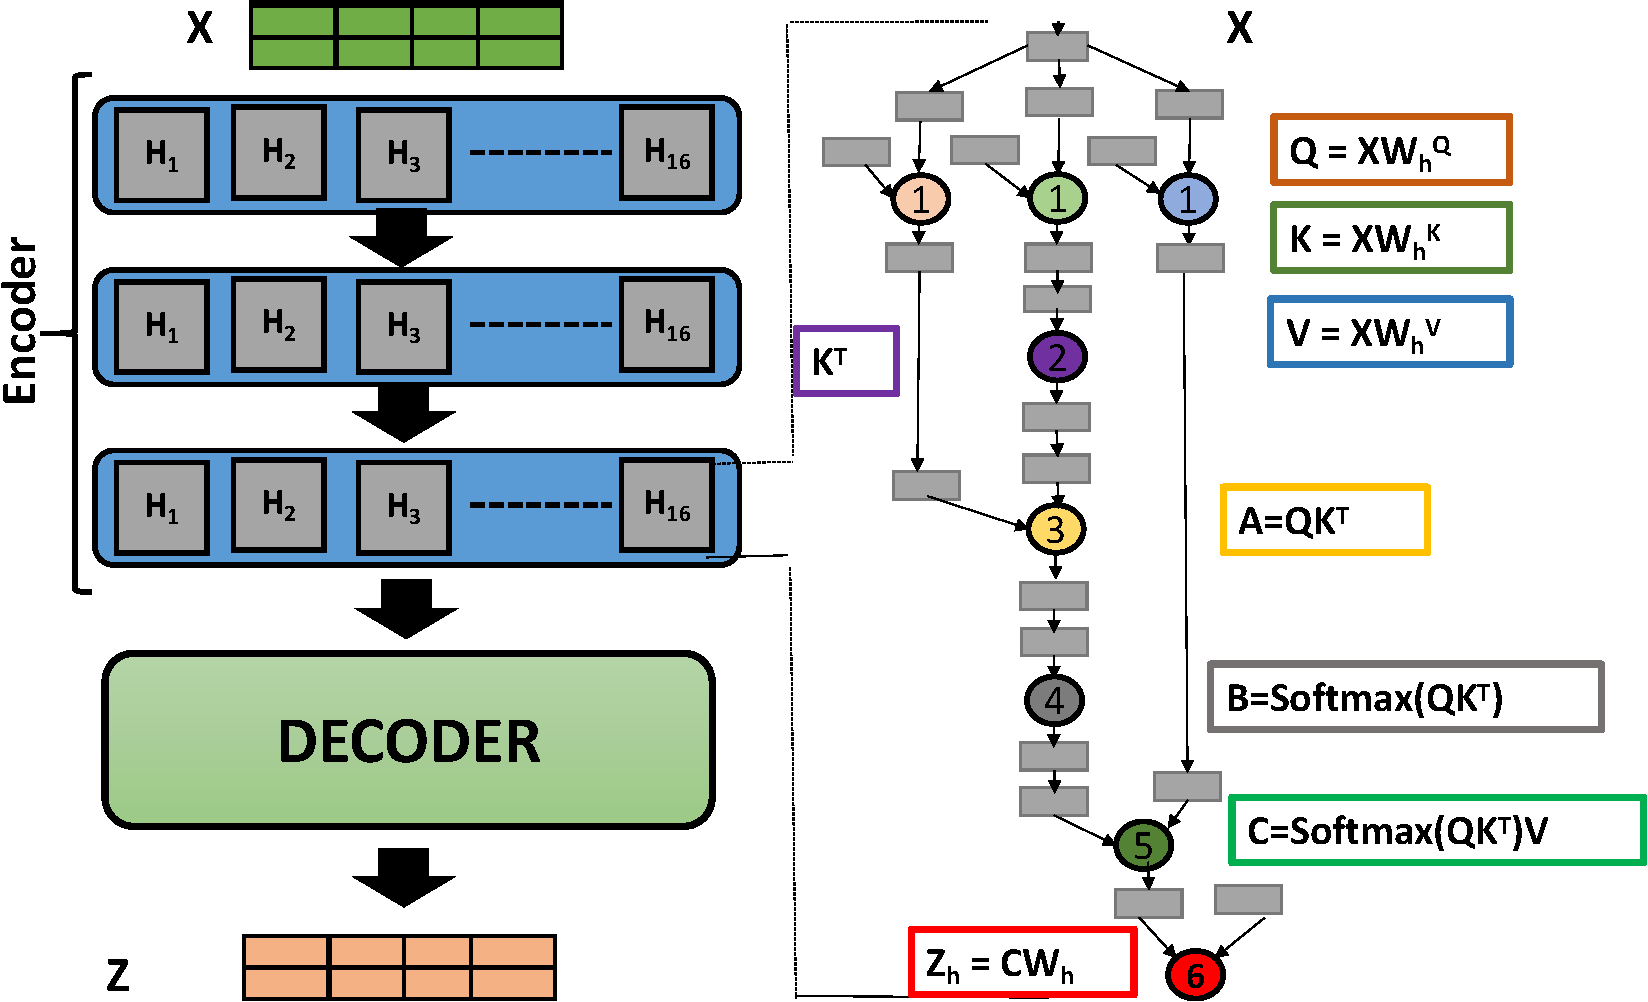
\includegraphics[scale=0.325]{Pictures/TransformerArch.pdf}
		\caption{\small Transformer Architecture\label{fig:transformer}}
	\end{figure}
	\par We conduct a series of experiments classified into three broad categories and for each experiment we define $\beta$ as the size of the transformer such that the matrices defined earlier $Q$,$K$,$V$,$X$ are all of dimensions $\beta \times \beta$. We denote the number of heads for the transformer as $H$. 
	\section{Experiment 1: Exhaustive Profiling}
	For Experiment 1, we profile one layer of the transformer architecture where we fix $\beta$ as 256 and vary the number of heads $H \in [1,16]$. Our experiment set is therefore a total of 16 input DAGs with each DAG representing a layer of a transformer neural network having $H\in[1,16]$ heads. 
	\par For each input DAG, we specify the task component mappings beforehand using the {\tt dev} guidance parameter for each kernel in the specification file. Given the structure of the DAG, it makes sense to cluster all kernels belonging to one transformer head into a task component and map it to a particular device. Since, the transformer heads are independent, such task component mappings would result in  there being no intra-edge buffers. As a result there will be no read callbacks. Thus for any transformer with $H$ heads, possible mapping configurations would be to 1) map all heads to a GPU device, 2) map 1 head to the CPU and $H-1$ heads to the GPU device, ... and finally $H+1$) mapping all $H$ heads to the GPU device.  Since each head is identical, clustering each head into a task component would result in a total of $H+1$ mapping configurations for a DAG with $H$ heads.
	\par We implement a static fine-grained scheduling heuristic called {\em clustering} specifically for any given transformer DAG with $H$ number of heads. Each task component $T_d$ represents one head and is annotated with the maximum bottom level rank defined in Equation \ref{eqn:brank_kernel} of the kernels in $FRONT(T_d)$. The $select$ routine for {\em clustering }selects from a set of task components, the component that has the maximum rank. The bottom level rank for any kernel in a DAG represents the maximum time left to finish all kernels in the path starting from $k$ to the last task in the DAG. The procedure $schedule$ sets up $C_d$ command queues for each task component $T_d$ mapped to device $d$. The {\em clustering} scheme for the transformer DAG is therefore characterized by the architecture mapping configuration tuple $mc=\langle CQ_{gpu},CQ_{cpu},h_{cpu}\rangle$. The parameter $Q_{gpu}\in [0,5] $ denotes the number of command queues used for the GPU device for executing a task component. Similarly, $Q_{cpu} \in [0,5]$ represents the number of command queues used for the CPU device. By varying the number of command queues for the CPU and the GPU, we have a total of $5*5=25$  architectural configurations. The parameter $h_{cpu}$ represents  the number of task components to be mapped to the CPU device.  The remaining $H-h_{cpu}$ task components are mapped to the GPU device. We consider the default configuration to be the case when the entire DAG is mapped to the GPU device using a single command queue i.e. $mc=(1,0,0)$, which essentially represents a coarse-grained scheduling decision, since we are using only 1 command queue.
	\par  For each DAG distinguished by the number of heads $H$, the best mapping configuration for {\em clustering} is the one which gives the best  speedup with respect to time taken by the DAG to execute in its default configuration which is using 1 GPU device with 1 command queue i.e. $mc=(1,0,0)$. We profile a total of $(H+1)*5*5$ such mapping configurations for each transformer DAG with $H$ heads and highlight our observations in  Fig. \ref{fig:Expt1}. 
	\begin{figure}[ht]
		\centering
		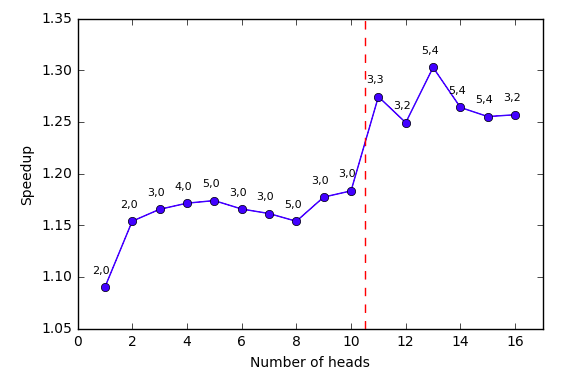
\includegraphics[scale=0.45]{Pictures/Expt-1.png}
		\caption{\small Speedup of best over default configuration \label{fig:Expt1}}
	\end{figure}
	The x-axis denotes the total number of heads for the transformer. The y-axis represents the speedups obtained for the best configuration for each DAG over the default configuration. Each point is labeled by the $CQ_{gpu},CQ_{cpu}$ tuple corresponding to the best configuration. We further note that for DAGs with number of heads upto 10 (region to the left of the dotted line), $h_{cpu}$ is 0. For DAGs having  number of heads greater than 10 (region to the right of the dotted line), we have $h_{cpu}=1$. 
	\par Thus, for DAGs with $H \in [1,10]$, we observe that the best configuration only differs from the default configuration with respect to the $CQ_{gpu}$ parameter. All the task components of the DAGs are scheduled to the GPU with the only difference being the number of command queues assigned to each component. The key observation in this region is that the transformer shows a clear speedup of about $15\% - 17\%$, if fine-grained scheduling is enabled leveraging multiple command queues. This highlights the effectiveness of automated fine-grained scheduling which our framework offers.
	\par For $H \in [11,16]$, we observe that scheduling one of the task components of the DAG to the CPU device yields the maximum speedups.  We also observe a jump in the relative speedup values as compared to the DAGs with $H <=10$. This is because apart from taking fine-grained scheduling decisions for the GPU device, we are also undertaking certain fine-grained scheduling decisions for the CPU device as well. This results in better extraction of application level-parallelism since mapping a task component to the CPU results in lesser contention for the GPU device. However, we observed that migrating more than one head does not yield better results. This may be attributed to the fact that overall execution of the transformer is bottlenecked by the time taken to execute kernels of a head on the CPU device. 
	\par We observe two key points from this experiment. Firstly, the transformer DAG is mapped efficiently using fine-grained scheduling decisions with the help of setting up multiple command queues, thereby lending credence to our framework's central idea of exploiting concurrency. Secondly, we observe that only for DAGs with $H > 10$, it is meaningful to utilise the CPU device for further speedups. This makes sense since i) the GPU has an order of magnitude number of processing elements greater than the CPU under consideration, ii) the kernels selected are optimized for GPUs rather than CPUs and iii) the CPU device is heavily engaged in setting up command queues and issuing directives to the devices in the heterogeneous platform.  Mapping more than 1 head for execution on the CPU actually takes more time to execute than that of mapping the remaining heads to the GPU device. 
	\par In the current experiment we consider specific DAG head mappings along with a choice of command queues and devices  based on what worked best for the given DAG and the given mapping configuration. Our next two categories of experiments consider typical dynamic heterogeneous scheduling policies like Eager-Scheduling and HEFT. We present a comparative evaluation between these methods and our clustering based static scheme in the context of the transformer DAG. 
		
	\section{Experiment 2: Clustering vs Eager Execution} We have implemented a simplistic eager execution based scheduling algorithm in our framework which is a dynamic scheduling scheme inspired from StarPU. For achieving this, we have implemented the $select$ routine to choose task components based on the bottom level ranks discussed earlier. Here, each task component represents one kernel in the DAG getting mapped to a device $d$ with one command queue.  For selecting devices, the $select$ routine selects any device that is available at runtime. Since, eager is a dynamic scheme, the choice of the device for execution is not known beforehand. This prohibits taking advantage of fine-grained scheduling decisions of interleaving data-transfers with execute operations.
	\begin{figure}[ht]
		\centering
		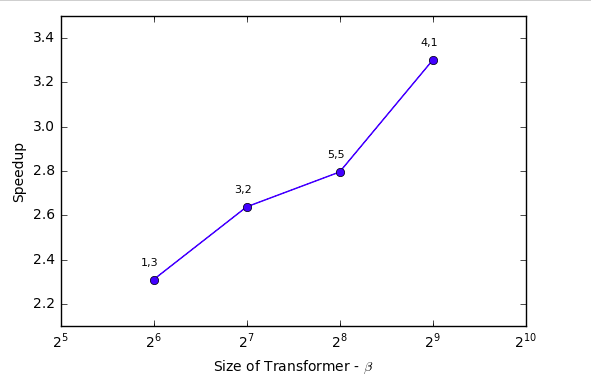
\includegraphics[scale=0.45]{Pictures/Expt-2.png}
		\caption{\small Clustering vs Eager \label{fig:Expt2}}
	\end{figure}
	\par For a comparative evaluation of this dynamic scheme with {\em clustering}, we generate a set of input DAGs by keeping the number of heads $H$ fixed to $16$ and by varying the size parameter $\beta$ from $64$ to $512$ in powers of 2. We profile each such input DAG, using both {\em eager} scheduling and {\em clustering} schemes for all possible mapping configurations. We compute the speedups of execution times taken by {\em clustering} based scheduling for the best mapping configuration  over that of {\em eager} and highlight them in Figure \ref{fig:Expt2}. 
	The x-axis represents the size of the transformer head ($\beta$) and the y-axis represents the speedup values. Each point in the plot is again labelled by the tuple $Q_{gpu},Q_{cpu}$ used by the best mapping configuration for the clustering scheme. The third element of the best configuration $H_{cpu}$ was found to be 1 for each $\beta$. It can be observed that {\em clustering} outperforms {\em eager} by a considerable margin. Since only one command queue per device is used, the scheduling scheme is restricted to taking coarse-grained scheduling decisions only and fails to take advantages of concurrency offered by fine-grained scheduling decisions. 
	\par We next perform a deeper analysis of the scheduling decisions taken by the two scheduling schemes for a DAG with $\beta=512$ using the Gantt charts for {\em eager} and {\em cluster} scheduling depicted in
	Figures \ref{fig:heft_gannt} and \ref{fig:best_gannt} respectively. The primary reason for the poor performance of  {\em eager} maybe attributed to the
	greedy nature of its dispatching mechanism. One can observe that multiple GEMM kernels have been scheduled on the CPU, thereby taking a significantly larger amount of time. The delay in  execution of the GEMM kernels in the first level stalls the entire progress of the DAG. 
	\section{Experiment 3: Clustering vs HEFT}
	We implement the standard Heterogeneous Earliest Finishing Time First algorithm using our framework whose primary principle is based on selecting kernels based on their bottom level ranks and dispatching to devices according to their estimated earliest finish times. Similar to {\em eager}, the scheduling heuristic {\em heft} assumes each task component to represent one kernel and sets up one command queue for each device. We override the $select$ routine such that each dispatch decision involves i) choosing the kernel $k$ with the maximum bottom level rank and for ii) choosing the device $d$ with the earliest finishing time (EFT). In our implementation, we calculate EFT of a device $d$ as the sum of the execution time of the kernel currently executing on $d$ and the execution time of the kernel to be dispatched on the device. Note, our implementation for HEFT is not calibrated to take into account scheduling overheads such as enqueuing delays while selecting devices. We again consider the same set of input DAGs used in Experiment 2 and plot the speedups of the best configurations of the clustering scheme over the {\em heft} scheme in  Figure \ref{fig:Expt3}.
	\begin{figure}[ht]
		\centering
		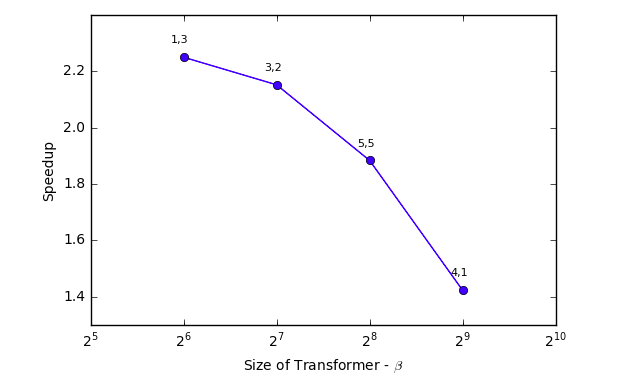
\includegraphics[scale=0.45]{Pictures/Expt-3.png}
		\caption{\small Clustering vs {\em heft} scheduling \label{fig:Expt3}}
	\end{figure}
	\par As expected, {\em heft} performs better than {\em eager} due to the prediction of earliest finishing times for each task.  However, {\em heft} being implemented as a dynamic scheme is short sighted and fails to exploit concurrency aware scheduling decisions undertaken by {\em clustering}. 
	\par We again perform a deeper analysis here between the scheduling decisions by plotting the Gantt chart for the DAG with $\beta = 512$ in Fig. \ref{fig:heft_gannt}. In contrast to {\em eager} scheduling, {\em heft} exclusively uses the GPU for the GEMM kernels and it thus approximately $2.4 \times$ faster than eager. 
	\par We next list a set of general observations explaining as to why our static clustering scheme performed better than that of the dynamic schemes {\em eager} and {\em heft}. From the gantt charts we may observe that kernels scheduled using our {\em clustering} scheme start much later when compared to kernels being scheduled in the other schemes. This may be attributed to the fact, that our framework sets up the command queues first with operations pertaining to all kernels in a task component  before actually scheduling the kernels to their respective devices. As a result, we can see that there exist no gaps between the execution of two kernels in our scheduling scheme.
	For the other two policies, despite being dynamic in nature, they have to rely on read callbacks to make dispatch decisions. Naturally, since read callbacks perform exclusive thread-safe updates, the successor kernels need to wait before getting dispatched. Furthermore, we can observe the gaps for the kernels scheduled to the GPU device to be more. This makes sense, since the callback function is initiated as a daemon thread by the OpenCL runtime system. The scheduler thread may be swapped out of main memory at that point of time by the operating system. The scheduler thread must resolve these updates first before dispatching the successor kernels. The successive gaps introduced between each kernel execution in the DAG results in a considerable slowdown when compared to the scheduling decisions employed by {\em clustering}. 
	\begin{figure}[ht]
		\centering
		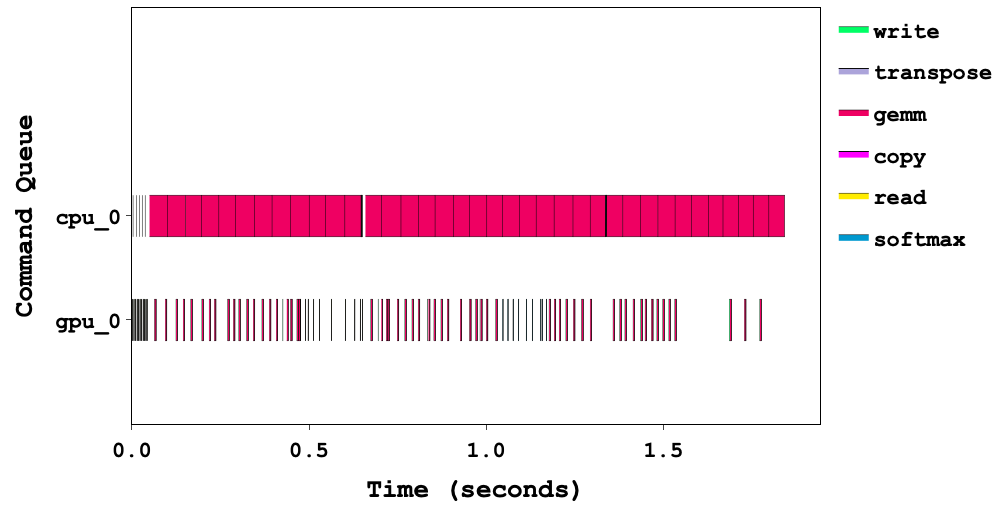
\includegraphics[scale=0.40]{Pictures/eager_gannt.png}
		\caption{\small Gannt chart for {\em eager} scheduling \label{fig:eager_gannt}}
	\end{figure}
	\begin{figure}[ht]
		\centering
		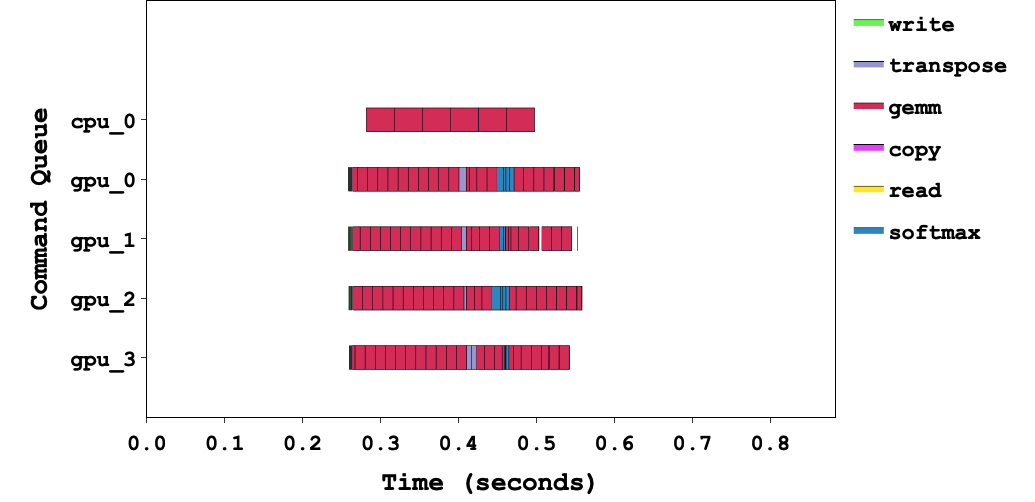
\includegraphics[scale=0.40]{Pictures/best_gannt.png}
		\caption{\small Gannt chart for {\em cluster} scheduling  \label{fig:best_gannt}}
	\end{figure}
	\begin{figure}
		\centering
		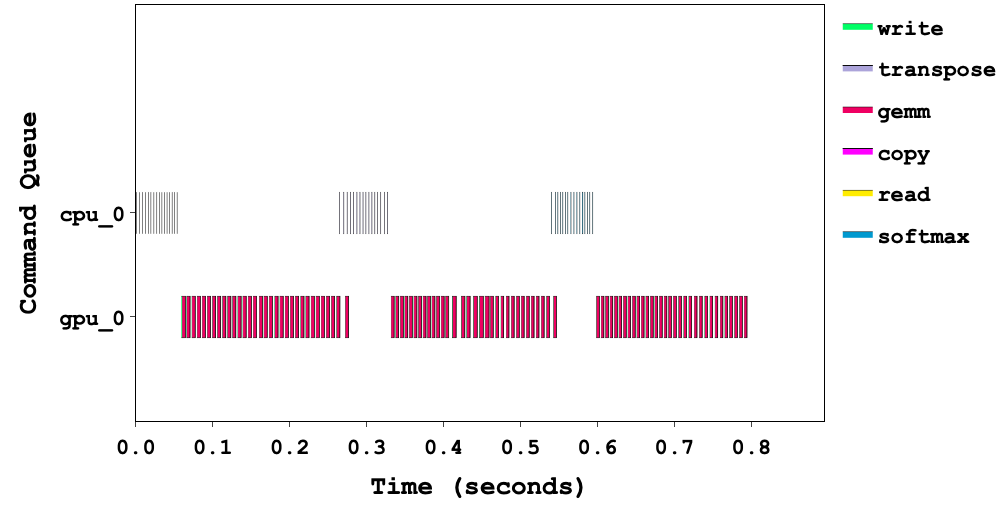
\includegraphics[scale=0.40]{Pictures/dynamic_heft_gannt.png}
		\caption{\small Gannt chart for {\em heft} scheduling \label{fig:heft_gannt}}
	\end{figure}
	Thus, we empirically establish the necessity for static cluster based scheduling policies for the transformer neural networks using these experiments. In general, for any application exhibiting potential scope for concurrency, scheduling schemes must be envisaged that take into account i)fine-grained scheduling decisions with respect to the structure of the DAG as well as ii) intricate runtime environment delays occurring as a result of enqueuing commands and processing simultaneous callback events.  
% Chapter Template

\chapter{Conclusion} % Main chapter title

\label{Chapter7} % Change X to a consecutive number; for referencing this chapter elsewhere, use \ref{ChapterX}

\lhead{Chapter 7. \emph{Conclusion}} % Change X to a consecutive number; this is for the header on each page - perhaps a shortened title

%----------------------------------------------------------------------------------------
%	SECTION 1
%----------------------------------------------------------------------------------------

We propose a platform agnostic scheduling framework that not only enables users to design HPC applications with ease, but also performs optimized scheduling decisions that exploit both application-level and platform-level concurrency. For an application with ample scope for concurrency, we showcased the utility of leveraging simple fine-grained static scheduling algorithms over dynamic coarse-grained scheduling algorithms. Currently, the framework lacks the notion of performance models which is beneficial for taking well informed scheduling decisions. Our future endeavours include exploring different scheduling algorithms that leverage Machine Learning based predictive modelling techniques to enrich the current set of scheduling decisions available in our framework. 

%----------------------------------------------------------------------------------------
%	THESIS CONTENT - APPENDICES
%----------------------------------------------------------------------------------------

\addtocontents{toc}{\vspace{2em}} % Add a gap in the Contents, for aesthetics

\appendix % Cue to tell LaTeX that the following 'chapters' are Appendices

% Include the appendices of the thesis as separate files from the Appendices folder
% Uncomment the lines as you write the Appendices

%% Appendix Template

\chapter{Appendix A} % Main appendix title

\label{AppendixX} % Change X to a consecutive letter; for referencing this appendix elsewhere, use \ref{AppendixX}

\lhead{Appendix X. \emph{Appendix Title Here}} % Change X to a consecutive letter; this is for the header on each page - perhaps a shortened title

Write your Appendix content here.

%\input{Appendices/AppendixB}
%\input{Appendices/AppendixC}

\addtocontents{toc}{} % Add a gap in the Contents, for aesthetics

\backmatter

%----------------------------------------------------------------------------------------
%	BIBLIOGRAPHY
%----------------------------------------------------------------------------------------
%\nocite{*}
\label{Bibliography}

\lhead{\emph{Bibliography}} % Change the page header to say "Bibliography"

\bibliographystyle{apalike} % Use the "custom" BibTeX style for formatting the Bibliography

\bibliography{Bibliography} % The references (bibliography) information are stored in the file named "Bibliography.bib"

\end{document}  
